% =====================================================================
%  Parameter-Efficient Deepfake Detection: Complete Research Journey,
%  Mathematical Foundations, Architecture, Implementation and
%  Experimental Results
%
%  Source of every number: the executed notebooks M0-M9b in this
%  repository (outputs as committed up to 06aedba, 5 Nov 2026).
%  Compile with:  tectonic complete_research_progress_report.tex
% =====================================================================
\documentclass[10pt,a4paper]{article}

\usepackage[a4paper,margin=2.1cm,headheight=14pt]{geometry}
\usepackage{lmodern}
\usepackage{amsmath,amssymb,bm}
\usepackage{booktabs,tabularx,longtable,multirow,array}
\usepackage{graphicx}
\usepackage{float}
\usepackage[font=small,labelfont=bf,skip=4pt]{caption}
\usepackage{xcolor}
\usepackage{enumitem}
\usepackage{fancyhdr}
\usepackage{tikz}
\usetikzlibrary{arrows.meta,positioning,fit,calc,shapes.geometric,backgrounds}
\usepackage[hidelinks]{hyperref}
\usepackage{microtype}

\setlist{itemsep=1pt,topsep=3pt,parsep=0pt}
\setlength{\parskip}{3pt}
\setlength{\parindent}{0pt}
\setlength{\emergencystretch}{3em}
\renewcommand{\arraystretch}{1.12}
\newcolumntype{Y}{>{\raggedright\arraybackslash}X}
\newcolumntype{R}{>{\raggedleft\arraybackslash}X}
\newcolumntype{L}[1]{>{\raggedright\arraybackslash}p{#1}}

\definecolor{done}{HTML}{1B7F3B}
\definecolor{fail}{HTML}{B22222}
\definecolor{part}{HTML}{B8860B}
\definecolor{plan}{HTML}{4A4A9A}
\definecolor{box}{HTML}{EEF2F7}
\definecolor{trn}{HTML}{FCE9C8}
\definecolor{frz}{HTML}{DCE6F2}
\newcommand{\Done}{\textcolor{done}{\textbf{completed}}}
\newcommand{\Fail}{\textcolor{fail}{\textbf{failed}}}
\newcommand{\Part}{\textcolor{part}{\textbf{partial}}}
\newcommand{\Plan}{\textcolor{plan}{\textbf{planned}}}
\newcommand{\Unv}{\textcolor{fail}{\textbf{unverified}}}
\newcommand{\NR}{\textit{not recorded}}
\newcommand{\figdir}{figures}

\pagestyle{fancy}
\fancyhf{}
\fancyhead[L]{\small\itshape Parameter-Efficient Deepfake Detection --- Research Record}
\fancyhead[R]{\small\itshape GBLA project, NIT Rourkela}
\fancyfoot[C]{\small\thepage}
\renewcommand{\headrulewidth}{0.4pt}

\begin{document}

% ---------------------------------------------------------------------
% COVER
% ---------------------------------------------------------------------
\begin{titlepage}
\centering
\vspace*{1.2cm}
{\large Research Project Technical Record \par}
\vspace{0.8cm}
\rule{\linewidth}{1pt}\par\vspace{0.4cm}
{\LARGE\bfseries Parameter-Efficient Deepfake Detection:\\[4pt]
Complete Research Journey, Mathematical Foundations,\\[4pt]
Architecture, Implementation and Experimental Results\par}
\vspace{0.4cm}\rule{\linewidth}{1pt}\par
\vspace{0.8cm}
{\large Generator-Balanced Latent Adaptation (GBLA) project\par}
\vspace{1.4cm}
{\large Satyabrata Mishra (225CS2022)\\ M.Tech, Computer Science and Engineering\par}
\vspace{0.4cm}
{\large Supervisor: Prof.\ Shyamapada Mukherjee\par}
\vspace{0.4cm}
{\large Department of Computer Science and Engineering\\
National Institute of Technology Rourkela\par}
\vfill
\begin{minipage}{0.86\linewidth}\small
\textbf{Status of this document.} Record of the research stage that ends on 5 November 2026
(repository commit \texttt{06aedba}). Every number in this report was read from the executed
notebook outputs in the repository; items that could not be traced to a file are marked
\Unv{} and are not used as results. Nothing in the implementation, datasets or experiment
configurations was changed while preparing this report.
\end{minipage}
\vspace{0.8cm}

{\large 5 November 2026\par}
\end{titlepage}

% ---------------------------------------------------------------------
% ABSTRACT
% ---------------------------------------------------------------------
\section*{Executive Summary}
\addcontentsline{toc}{section}{Executive Summary}

\textbf{Goal.} Build a deepfake detector that (i) trains as few parameters as possible on top of a
frozen pretrained model and (ii) generalises to manipulation methods (``generators'') and datasets
not seen in training. The project is framed as \emph{parameter-efficient optimisation}: the
question is how to train a very small set of parameters so that the result transfers, not how to
compress a representation or a weight manifold.

\textbf{What was built and run (M0--M9b, 5 Oct -- 5 Nov 2026).}
A frozen OpenAI CLIP ViT-L/14 visual encoder (303,181,826 parameters in the detector) in which only
the 50 LayerNorms and a linear head on the L2-normalised 1024-d CLS token are trained:
\textbf{104,450 trainable parameters (0.0345\%)}. On FaceForensics++ c23 this baseline (a
reproduction of LNCLIP-DF \cite{yermakov2025lnclip}) reaches 98.04 seen-generator video AUC and
88.37 on the unseen FaceShifter generator, within 0.8 points of the published numbers on every
test set. Two attempts to shrink the trainable set further by a seeded random-subspace latent
(\(\theta=\theta_0+\alpha Wz\), M2/M2b) \textbf{failed}: with \(d\le 1024\) the latent learned
little beyond the class ratio or the head alone. A curvature-based explanation of
generator dominance (M3) also \textbf{failed} its own checks, although a geometric measurement showed
that pooled training is dominated by Face2Face and nearly ignores NeuralTextures.

The method that survived is \textbf{GBLA}: during training each generator \(g\) uses
\(\theta_s+\delta_g\) with a penalty \(\lambda\|\delta_g\|^2\), batches are pure (one generator at a
time) and only the shared \(\theta_s\) (104,450 numbers) is deployed. With \(\lambda=0.01\):
\begin{itemize}
\item FaceShifter (unseen, FF++) video AUC \textbf{92.91} vs 90.53 for pooled training with the
same batching and 88.19 for the LNCLIP-DF reproduction at the same 10-epoch budget;
\item leave-one-generator-out mean held-out AUC \textbf{88.04} vs 87.49 pooled and 85.34 for a
Fisher merge, but \emph{worse} when NeuralTextures is held out (62.29 vs 64.40);
\item cross-dataset DFD video AUC \textbf{96.71} [95.30, 98.21] vs 95.88 for the reproduction
(paired difference \(+0.82\) [\(+0.02,+1.73\)]), and UADFV \textbf{99.63} vs 99.25 (difference not
significant; UADFV is near ceiling).
\end{itemize}
The parameter count of the deployed detector is unchanged from LN-tuning; GBLA changes how those
parameters are optimised. All results are single-seed.

\textbf{Reference values supplied for verification.} The total of 303,966,208 parameters is
verified, but it is the full ViT-L/14 visual tower \emph{including} the unused 786,432-parameter
text projection (M0). The value ``786,432 trainable (0.2587\%)'', the LoRA adapters on
\texttt{q\_proj}/\texttt{v\_proj}, the codebook utilisation (97/1024, 46/1024) and the
accuracy/loss figures (98.38\%, 97.56\%, 0.134335, 97.125\%) do not appear in any notebook, log,
commit or document of this project; no LoRA or codebook code exists. They are reported as
\Unv{} (Section~\ref{sec:verify}).

\clearpage
\tableofcontents
\clearpage
\listoffigures
\listoftables
\clearpage

% =====================================================================
\section{Research Motivation and Problem Formulation}\label{sec:motivation}
% =====================================================================

\subsection{Why deepfake detection matters}
Face-manipulation tools can replace identities (face swapping) or re-enact expressions in real
videos. Detectors are needed wherever video is used as evidence or to inform the public. The
practical difficulty is not detecting a known manipulation method; it is detecting a method that
was not available when the detector was trained.

\subsection{Limitations of conventional detectors}
\begin{itemize}
\item \textbf{Generator-specific artifacts.} A detector trained on a few manipulation methods
(generators) learns cues that are specific to them, for example blending seams or texture
statistics. Same-generator accuracy on FaceForensics++ (FF++) \cite{rossler2019ffpp} is close to
saturation and hides this weakness.
\item \textbf{Generalisation gaps.} Accuracy on an unseen generator, or on a different dataset with
other capture conditions and compression, is usually much lower. Two kinds of shift must be
kept apart: \emph{cross-generator} (same dataset, new manipulation method) and
\emph{cross-dataset} (new data source).
\item \textbf{Cost of fine-tuning large models.} Large pretrained backbones such as CLIP
\cite{radford2021clip} transfer better than small CNNs, but fine-tuning all of their roughly 303 M
parameters is expensive, needs much memory for optimiser state, and can overfit to the training
generators.
\end{itemize}

\subsection{Research objective}
\begin{quote}
\emph{Develop a parameter-efficient deepfake detection framework that minimises the number of
trainable parameters while retaining detection performance and improving generalisation across
different deepfake generation methods.}
\end{quote}
The intent is to keep the representational power of a frozen pretrained model and adapt only a
very small set of parameters. Throughout this report, ``parameter-efficient'' means a small number
of \emph{trained and stored} parameters. The frozen backbone is still part of the model and is
always reported (Total / Trainable / Frozen / Trainable\%). Inference compute is not reduced by
any method in this project.

\subsection{How the objective evolved}\label{sec:evolution-short}
\begin{enumerate}
\item \textbf{Literature phase (24--29 Sep 2026).} Five papers were analysed (Section~\ref{sec:lit}).
The common assumption that ``fewer trainable parameters \(\Rightarrow\) better generalisation'' was
found to be contradicted by LNCLIP-DF's own LoRA result, and generator dominance in pooled training
was identified as an unmeasured quantity.
\item \textbf{Initial proposal (29 Sep -- 1 Oct).} ``One Generator, One Vote'': measure how unequally
generators influence pooled training (effective number \(G_\text{eff}\)) and rebalance them, all
inside a tiny seeded latent so that the deployed adaptation would be about 65 numbers. The method
name GBLA (Generator-Balanced Latent Adaptation) dates from this stage.
\item \textbf{Compact latent abandoned (M2/M2b, 14--15 Oct).} The latent could not represent the
LayerNorm adaptation at small \(d\) (Section~\ref{sec:m2}). The compact-payload claim was dropped.
\item \textbf{Curvature explanation abandoned (M3, 17 Oct).} The Hessian-based weighting did not
explain the pooled solution; only the geometric dominance measurement survived.
\item \textbf{Current method (M4 onward, 17 Oct -- 5 Nov).} GBLA as shared-plus-private
optimisation directly on the 104,450 LayerNorm and head parameters, evaluated by
leave-one-generator-out (M5), against merging baselines (M6), and across datasets (M8b, M9b).
\end{enumerate}
The mid-semester report and slides of 3 November 2026 still describe stage~2 (latent,
65 deployed numbers, ``progress up to M2'') although M3--M7 had been run by 20 October. That
document is therefore out of date with respect to the method; this report supersedes it.

% =====================================================================
\section{Sources, Investigation Method and Chronology}\label{sec:sources}
% =====================================================================

\subsection{What exists in the workspace}
The investigation covered the workspace \texttt{E:\textbackslash NITR\textbackslash 3rd Semester\textbackslash Satyabrata Research},
the git history of the repository, the paper folder, the mid-semester folder and the project
conversation record.

\begin{table}[H]\centering\small
\caption{Inventory of project artefacts examined.}\label{tab:inventory}
\begin{tabularx}{\linewidth}{@{}L{4.6cm}Y@{}}
\toprule
Artefact & Content and use in this report\\
\midrule
Repository notebooks \texttt{M0.ipynb} \dots\ \texttt{M9b.ipynb} & 14 executed notebooks (M0, M1, M2, M2b, M3, M4, M5, M6, M7, M7b, M8a, M8b, M9a, M9b), each holding code, configuration and outputs. \textbf{Primary source of every number.}\\
Git history (16 commits) & Dates and order of milestones (Table~\ref{tab:chronology}).\\
\texttt{unzip\_dfd\_c23.ipynb},\newline \texttt{unzip\_celebdf\_v2.ipynb} & Dataset download/unzip helpers outside the repository; not part of the research pipeline.\\
\texttt{Thesis Papers/} (8 PDFs) & Papers 4--8 analysed in the literature phase; papers 1--3 are background (Transformer, PCA tutorial, Transformer slides).\\
Mid-semester GBLA report (PDF) and two slide decks (\texttt{.pptx}) & Earlier GBLA documentation (state up to M2).\\
\texttt{Mid Semester/}\newline\texttt{RP\_MID\_SEM/} & A separate multimodal (audio-visual) project report and proxy-task metrics; \emph{not} part of this project. It is the only place where Tian et al.\ \cite{tian2023unsupervised} is cited.\\
Project conversation record & Literature analysis, design decisions, bugs and their fixes.\\
\midrule
Not present & No \texttt{.py} modules, no README, no training logs outside notebooks, no checkpoints in the repository (checkpoints stay on C-DAC under \texttt{runs/}), no LoRA or codebook code.\\
\bottomrule
\end{tabularx}
\end{table}

\textbf{Verification policy.} A number is reported as a result only if it appears in an executed
notebook output. Where a quantity was planned but never measured, it is marked \Plan{} or
\NR. Where a value was supplied from earlier discussion but has no source file, it is marked
\Unv.

\subsection{Chronology}
\begin{table}[H]\centering\small
\caption{Chronology reconstructed from the conversation record and the git log.}\label{tab:chronology}
\begin{tabularx}{\linewidth}{@{}L{2.2cm}L{1.6cm}YL{1.7cm}@{}}
\toprule
Date (2026) & Commit & Activity & Status\\
\midrule
24 Sep & -- & Analysis of papers 4--8 (Section~\ref{sec:lit}); hypotheses A--F and candidates C1--C5 & \Done\\
29 Sep -- 1 Oct & -- & GBLA proposal (``One Generator, One Vote''), pipeline design, claims audit & \Done\\
5 Oct & \texttt{2572354} & Initial code (repository created) & \Done\\
8 Oct & \texttt{83cd5dc} & M0 data pipeline: 192,000 paired face crops & \Done\\
13 Oct & \texttt{3e62dfe} & M1 LNCLIP-DF reproduction (20 epochs) & \Done\\
14 Oct & \texttt{dfc41db} & M2 latent re-parameterisation of LN + head, \(d\in\{16,\dots,4096\}\) & \Fail\\
15 Oct & \texttt{6549a0e} & M2b latent LN with directly trained head & \Fail\\
17 Oct & \texttt{9f1d12d} & M3 E1 go/no-go: per-generator solutions, curvature, \(G_\text{eff}\) & NO-GO (curvature)\\
18 Oct & \texttt{0ef0d1f} & M4 GBLA \(\lambda\) sweep & \Done\\
19 Oct & \texttt{0731e63} & M5 leave-one-generator-out (LOGO) at \(\lambda=0.01\) & \Done\\
19 Oct & \texttt{04aa840} & M6 Fisher / uniform merge baselines & \Done\\
20 Oct & \texttt{5ef28c8}, \texttt{7a6758d} & M7 \(G_\text{eff}\) law over 25 subsets; M7b re-analysis & \Done{} (law not supported)\\
3 Nov & -- & Mid-semester report and slides (describe state up to M2) & superseded\\
4 Nov & \texttt{439e77a}, \texttt{6661977} & M8a DFD preprocessing; M8b DFD cross-dataset test & \Done\\
5 Nov & \texttt{f8f6bb7}, \texttt{06aedba} & M9a UADFV preprocessing; M9b UADFV cross-dataset test & \Done\\
\bottomrule
\end{tabularx}
\end{table}

% =====================================================================
\section{Literature Review}\label{sec:lit}
% =====================================================================

The literature phase started on 24 September 2026 with papers 4--8 of the thesis paper folder.
Files 7 and 8 are two versions of the same work (LNCLIP-DF), so four distinct contributions were
analysed. Tian et al.\ (Paper~1 in the task specification) is not part of that set; it appears only
in a separate audio-visual project report stored in the same mid-semester folder. It is reviewed
here because it was requested, with its bibliographic details verified against the arXiv record.
No ``CVPR 2025 generalisable video-based deepfake detection'' paper appears anywhere in the project
record, so none is reviewed. Statements below about a paper's content are limited to what was read
from the paper during the literature phase or, for Tian et al., from the arXiv text.

\subsection{Paper 1 --- Tian et al., unsupervised multimodal detection}\label{sec:tian}
\textbf{Citation.} M.~Tian, M.~Khayatkhoei, J.~Mathai, W.~AbdAlmageed, ``Unsupervised Multimodal
Deepfake Detection Using Intra- and Cross-Modal Inconsistencies'', arXiv:2311.17088, 2023
\cite{tian2023unsupervised}. A later version appeared at BMVC 2025 under the title ``Unsupervised
Multimodal Deepfake Detection Through Explicit Intra-Modal and Cross-Modal Inconsistency
Discovery''.

\textbf{Problem and motivation.} Supervised detectors need labelled fakes and do not generalise to
new generation methods. The authors detect deepfake videos without fake training data by finding
inconsistencies inside a single video.

\textbf{Method.} The central hypothesis is that motion-transfer deepfakes face a trade-off: if the
motion of the source is transferred exactly, identity becomes inconsistent across frames; if
identity is kept exact, motion is distorted and no longer matches the audio. They support this with
an experiment in which identity is predicted from facial-landmark motion vectors, which works much
better on real than on fake videos. Two scores are computed over time windows of a video:
an \emph{intra-modal} identity-consistency score (similarity of identity features of the same video
across windows) and a \emph{cross-modal} audio--video consistency score (similarity between audio
and visual features of the same window). Networks are trained with consistency losses built from
similarity matrices across identities and time windows, on real VoxCeleb2 videos only.

\textbf{Results (as reported).} Average AUC 96.81\% on FakeAVCeleb, above prior unsupervised
methods; trained only on VoxCeleb2 with FakeAVCeleb identities removed.

\textbf{Strengths and limitations.} No fake data in training, explainable (localises inconsistent
windows), no per-identity reference video. It needs audio and talking-face video and is designed
for motion-transfer fakes; it does not address single-frame face images.

\textbf{Relation to this project.} None of its components were adopted. GBLA is a visual-only,
frame-level, supervised method. The idea of training without fake labels was considered in the
literature phase through the audio paper CA-SOADD (candidate C3 below), not through this paper.
Exact loss equations of this paper are not reproduced here because they were not part of the
project analysis.

\subsection{Paper 4 --- Mapping Networks (Sen \& Mukherjee)}\label{sec:mapping}
\textbf{Citation.} L.~Sen, S.~Mukherjee, ``Mapping Networks'', CVPR 2026 \cite{sen2026mapping}
(NIT Rourkela).

\textbf{Objective and method.} Replace training of a high-dimensional weight vector by training a
small latent \(z\in\mathbb{R}^d\) that generates the weights through a fixed mapping:
\(\hat\theta=\sigma(Wz+b)\), \(W\in\mathbb{R}^{P\times d}\), with a Mapping Loss
\(L_\text{map}=L_\text{task}+\lambda_\text{st}L_\text{stab}+\lambda_\text{sm}L_\text{smooth}+\lambda_\text{al}L_\text{align}\).
Deepfake detection is one of five demonstration tasks.

\textbf{Observations made in the project analysis.} (i) Trainable parameters are tiny (e.g.\ 2,048),
but the fixed mapping matrix must be stored: for a 537,994-parameter target network and
\(d=2048\), \(|W|\approx1.10\times10^9\) entries (about 4.4 GB in fp32), which the paper does not
report. (ii) With the stated modulation \(w_{ij}\leftarrow w_{ij}+\alpha z_i\), the added term is
\(\alpha\|z\|^2\), the same for every output index, so ``weight modulation'' adds a single shared
scalar. (iii) Deepfake results are same-dataset accuracies (Celeb-DF, FF++) with no cross-generator
or cross-dataset test.

\textbf{Adopted / not adopted.} The \emph{idea} of training a low-dimensional latent that generates
parameters inspired the M2/M2b latent re-parameterisation, applied only to the 104,450 LayerNorm and
head parameters and with an explicit offset \(\theta_0\) and a seeded (not stored) \(W\). That
experiment failed (Section~\ref{sec:m2}). The non-linearity \(\sigma\), the modulation and the Mapping
Loss terms were not adopted. In the final framing Mapping Networks is related work, not the basis of
the method.

\subsection{Paper 5 --- Breaking Manifold Continuity (Wang et al.)}
\textbf{Citation.} C.~Wang, J.~Wang, K.-Y.~Zhang, T.~Yao, S.~Ding, R.~Yi, L.~Ma, ``Breaking
Manifold Continuity: Vector Quantized Modeling for Real-Centric Deepfake Detection'', ICML 2026
(PMLR) \cite{wang2026breaking}.

\textbf{Method.} A learnable codebook (\(K=1024\), \(D=1024\)) quantises CLIP ViT-L/14 patch tokens;
a 2-block masked ViT restores context; per-code tangent bases \(U_k\in\mathbb{R}^{1024\times16}\)
separate valid real variation from off-manifold residuals; a hypernetwork conditioned on the CLS
token fuses the residuals. Training uses FF++ c23 with 8 frames per video; testing uses 32 frames
per video on six datasets and six DF40 methods.

\textbf{Parameter accounting verified in the analysis.} Codebook \(1024\times1024=1{,}048{,}576\);
tangent bases \(1024\times1024\times16=16{,}777{,}216\); total trainable about 45.34 M of 348.53 M
(13.0\%).

\textbf{Adopted / not adopted.} Nothing was implemented. The 8-frame training / 32-frame testing
protocol of this paper is the origin of the ``8 frames'' setting mentioned in the project; this
project trains and tests on 32 frames per video and subsamples 8 frames only for validation
monitoring (Section~\ref{sec:frames}). The codebook idea is the only codebook in the project
record, and it was never implemented (Section~\ref{sec:codebook}).

\subsection{Paper 6 --- CA-SOADD (Zhao et al.)}
\textbf{Citation.} Y.~Zhao, K.~Zhang, Z.~Hua, Y.~Zhang, Q.~Liao, W.~Jiang, ``Learning Tight Rejection
Boundaries without Negatives for Strict One-Class Audio Deepfake Detection'', ICML 2026 (PMLR)
\cite{zhao2026casoadd}.

\textbf{Method.} Strict one-class audio detection: real-only training, a non-learnable running
centroid \(c\), compactness \(1-\cos(z,c)\), benign-invariance, and a centroid-anchored margin
\(\max(0,m-\cos(z,c)+\cos(z^-,c))\) against structure-disrupting probes \(z^-\); online
standardisation; leave-one-family-out evaluation.

\textbf{Adopted / not adopted.} Not implemented. Its leave-one-family-out protocol motivated the
leave-one-generator-out evaluation of M5. A real-only image variant (candidate C3) was proposed in
the analysis but not pursued.

\subsection{Papers 7/8 --- LNCLIP-DF / GenD (Yermakov et al.)}
\textbf{Citations.} A.~Yermakov, J.~Cech, J.~Matas, M.~Fritz, ``Deepfake Detection that Generalizes
Across Benchmarks'', arXiv:2508.06248, 2025 \cite{yermakov2025lnclip} (the M1 notebook records the
venue as WACV 2026 and the code as \texttt{github.com/yermandy/GenD}); and the earlier version
A.~Yermakov, J.~Cech, J.~Matas, ``Unlocking the Hidden Potential of CLIP in Generalizable Deepfake
Detection'', arXiv:2503.19683 \cite{yermakov2025unlocking}.

\textbf{Method.} Frozen CLIP ViT-L/14; only LayerNorm affine parameters and a linear head on the
L2-normalised CLS token are trained (104,450 parameters, 0.03\%); loss
\(L_\text{CE}+0.1L_\text{align}+0.5L_\text{unif}\) (alignment/uniformity of Wang \& Isola
\cite{wang2020alignment}); optional slerp latent augmentation; paired real/fake training data;
RetinaFace crops with landmark alignment at 256 px.

\textbf{Reported results used as reference.} arXiv v1 Table~3 (video AUROC): FF 98.0, DF 99.6, F2F
98.2, FS 98.6, NT 95.7, FaceShifter 88.2 (87.3 without slerp, Table~5). GenD CLIP Table~4: DFD
96.4, UADFV 99.2, FaceShifter 86.6 (means of 5 seeds).

\textbf{Adopted.} The whole baseline recipe (backbone, trainable set, loss, optimiser schedule,
augmentations, real/fake pairing) is adopted unchanged in M1 and kept in every later experiment.
\textbf{Not adopted.} RetinaFace alignment (MTCNN boxes used instead), the external validation mix
(FF++ val used), slerp augmentation, multiple seeds.

\subsection{Other works used by the method or found in novelty checks}
\begin{itemize}
\item \textbf{Used directly:} FF++ \cite{rossler2019ffpp}; FaceShifter \cite{li2020faceshifter};
DFD (Google/Jigsaw, distributed with FF++); UADFV \cite{yang2019uadfv}; MTCNN
\cite{zhang2016mtcnn}; CLIP \cite{radford2021clip}; alignment/uniformity \cite{wang2020alignment};
Fisher-weighted merging \cite{matena2022fisher}; Kish effective sample size \cite{kish1965};
leave-one-domain-out protocol in the spirit of DomainBed \cite{gulrajani2021domainbed}.
\item \textbf{Used as concepts:} intrinsic dimension / random-subspace training
\cite{li2018intrinsic,aghajanyan2021intrinsic}; seeded generation of weights (PRANC, NOLA)
\cite{nooralinejad2023pranc,koohpayegani2024nola}; shared-plus-specific decomposition
\cite{khosla2012undoing,evgeniou2004multitask,piratla2020csd}; random-effects meta-analysis
\cite{dersimonian1986meta} (an analogy, later dropped).
\item \textbf{Found in novelty checks} (recorded in the project conversation; titles and IDs as
recorded, content not re-verified for this report): S3 ``Suppressing Forgery-Specific Shortcuts''
(arXiv:2606.01843), FMSD (arXiv:2601.01041), RINE (arXiv:2402.19091), CSD, CDA (ICCV 2025), DF40
(NeurIPS 2024), ``Not All Attacks Are Learned Equally in Speech Deepfake Detection''
(arXiv:2609.11763), FedNova, ``Diversity over Uniformity'' (CVPR 2026), SAFE (AAAI). They shaped
which claims were \emph{not} made (e.g.\ gradient-subspace projection was already published in S3).
\end{itemize}

\subsection{Comparison}
\begin{table}[H]\centering\scriptsize
\caption{Literature comparison. ``Adopted'' = used unchanged; ``inspired'' = idea taken, implementation ours; ``none'' = not used.}\label{tab:litcomp}
\begin{tabularx}{\linewidth}{@{}L{1.9cm}L{2.3cm}L{1.9cm}L{1.9cm}YL{2.3cm}Y@{}}
\toprule
Paper & Main approach & Backbone & Trainable & Key mathematical idea & What we took & Limitations (as analysed)\\
\midrule
Tian et al.\ 2023 & Unsupervised intra-/cross-modal inconsistency & identity, video and audio networks & all networks (count not analysed) & consistency of identity over time and of audio vs video & none & needs audio; motion-transfer fakes; FakeAVCeleb only\\
Mapping Networks (CVPR'26) & weights generated from a latent & small CNNs, ResNet50 & latent \(z\) (\(\sim10^3\)) & \(\hat\theta=\sigma(Wz+b)\) & inspired M2/M2b latent (failed) & stores \(O(Pd)\) mapping; no cross-generator test\\
Breaking Manifold Continuity (ICML'26) & VQ codebook on real CLIP patch tokens + tangent residuals & CLIP ViT-L/14 + Effort & 45.34 M (13.0\%) & discrete bottleneck, \(\|(I-U_kU_k^\top)\Delta\|\) & none (8/32-frame protocol noted) & large trainable set; codebook size chosen on test sets\\
CA-SOADD (ICML'26) & strict one-class audio, centroid margin & frozen SSL speech encoder & not reported & \(\max(0,m-\cos(z,c)+\cos(z^-,c))\) & inspired LOGO protocol & audio only\\
LNCLIP-DF / GenD (arXiv'25, WACV'26) & LayerNorm tuning of frozen CLIP & CLIP ViT-L/14 & 104,450 (0.03\%) & L2-normalised CLS; CE + align + uniform & \textbf{adopted} as baseline and backbone of GBLA & external val set overlaps test datasets; mechanism of slerp unverified\\
\bottomrule
\end{tabularx}
\end{table}

% =====================================================================
\section{Evolution of the Research Architecture}\label{sec:arch-evolution}
% =====================================================================

\subsection{Initial ideas (literature phase)}
Six hypotheses (A--F) and five candidates (C1--C5) were written down on 24 September: an
adapter-geometry study (LN vs LoRA at matched size), a training-free real-manifold residual, a
real-only centroid detector, a latent-subspace adapter over LN space, and explicit
generator-invariance (rejected as already published). None of C1--C3 or C5 was implemented. C4
(latent over LN space) became the first GBLA design and was implemented in M2/M2b.

\subsection{Component decisions}
\begin{table}[H]\centering\scriptsize
\caption{Every architectural component considered, with purpose, dimensions and implementation status.}\label{tab:components}
\begin{tabularx}{\linewidth}{@{}L{2.3cm}YL{2.6cm}L{1.9cm}L{1.6cm}@{}}
\toprule
Component & Purpose and reason & Input \(\to\) output & Source & Status\\
\midrule
Face crop (MTCNN, 1.3\(\times\) square) & remove background; same box for real and fake & frame \(\to 224\times224\times3\) & \cite{zhang2016mtcnn} & \Done{} (M0)\\
CLIP ViT-L/14 visual encoder (frozen, QuickGELU) & transferable features without fine-tuning cost & \(3\times224\times224\to\mathbb{R}^{1024}\) (CLS after \texttt{ln\_post}) & \cite{radford2021clip} & \Done{} (M1--)\\
CLIP text projection (\(1024\times768\)) & not needed for a binary head & -- & -- & removed (786,432 params not counted)\\
LayerNorm affine (50 modules) & the only adapted backbone parameters; per-channel scale/shift cannot create new feature directions & \(\gamma,\beta\in\mathbb{R}^{1024}\) each & \cite{yermakov2025lnclip} & \Done{} (trainable)\\
L2 normalisation & hyperspherical features for align/uniform losses & \(\mathbb{R}^{1024}\to S^{1023}\) & \cite{yermakov2025lnclip} & \Done\\
Linear head & real/fake logits & \(1024\to2\) (2,050 params) & \cite{yermakov2025lnclip} & \Done\\
Seeded latent \(\theta=\theta_0+\alpha Wz\) & compress trainable set to \(d+1\) numbers & \(z\in\mathbb{R}^d\to\theta\in\mathbb{R}^{P}\) & \cite{li2018intrinsic,nooralinejad2023pranc,sen2026mapping} & \Fail{} (M2, M2b); removed\\
Shared \(\theta_s\) + private \(\delta_g\) (GBLA) & stop dominant generators from fixing the shared solution & \(\theta_s,\delta_g\in\mathbb{R}^{104{,}450}\) & our use of \cite{evgeniou2004multitask,piratla2020csd} & \Done{} (M4--)\\
Pure-generator round-robin batching & each step sees one generator and its own reals & block of 225 steps & ours & \Done{} (M3 sampler, M4--)\\
LoRA adapters & -- & -- & -- & \textbf{not implemented}\\
Codebook / vector quantisation & -- & -- & \cite{wang2026breaking} (literature only) & \textbf{not implemented}\\
Slerp latent augmentation & -- & -- & \cite{yermakov2025unlocking} & not used\\
\bottomrule
\end{tabularx}
\end{table}

\subsection{Why each major decision was taken}
\begin{itemize}
\item \textbf{CLIP ViT-L/14 with LayerNorm tuning.} It was the strongest published parameter-efficient
detector with exact, verifiable parameter accounting (104,450), and LayerNorm tuning cannot
synthesise new channel directions, which was argued to limit memorisation of generator artifacts.
\item \textbf{Latent re-parameterisation (tried, removed).} It was meant to reduce the deployed
adaptation to \(d+1\) numbers and to make generator balancing exact in a small space. M2/M2b showed
that \(d\le1024\) loses most of the adaptation (Section~\ref{sec:m2}).
\item \textbf{Shared plus private offsets.} M3 showed one generator (Face2Face) dominates pooled
training and one (NeuralTextures) is almost ignored. Private offsets let each generator fit its own
residual during training, while the deployed \(\theta_s\) is shared.
\item \textbf{No LoRA.} LNCLIP-DF reports that LoRA overfits quickly on this task; the project's
hypothesis was that the structure of the adaptation (diagonal vs low-rank mixing) matters. LoRA was
listed as a comparison (candidate C1) but never implemented.
\end{itemize}

% =====================================================================
\section{Mathematical Foundations}\label{sec:math}
% =====================================================================
Notation: \(x\) is a face crop, \(y\in\{0,1\}\) its label (1 = fake), \(g\in\mathcal{G}\) the generator
of a fake, \(G=|\mathcal{G}|\). Bold or capital letters denote matrices; \(P=104{,}450\) is the number
of adapted parameters.

\subsection{A. Feature extraction with the frozen CLIP ViT-L/14}\label{sec:clip}
\textbf{Pre-processing.} A \(224\times224\) RGB crop is scaled to \([0,1]\) and normalised per channel
with CLIP's mean \((0.48145466,0.4578275,0.40821073)\) and standard deviation
\((0.26862954,0.26130258,0.27577711)\): \(\tilde x=(x-\mu)/\sigma\in\mathbb{R}^{3\times224\times224}\).

\textbf{Patch embedding.} A convolution with kernel and stride 14 splits the image into
\(16\times16=256\) patches and maps each to 1024 dimensions:
\begin{equation}
E=\mathrm{Conv}_{14\times14}(\tilde x)\in\mathbb{R}^{1024\times16\times16}\;\Rightarrow\;
[e_1,\dots,e_{256}],\; e_i\in\mathbb{R}^{1024},
\end{equation}
with \(1024\cdot3\cdot14\cdot14=602{,}112\) weights (no bias), matching the M1 parameter report.

\textbf{Tokens and positions.} A learned class token \(c\) is prepended and learned positional
embeddings \(p_i\) are added, giving 257 tokens:
\begin{equation}
H^{(0)}=\mathrm{LN}_\text{pre}\big([c;e_1;\dots;e_{256}]+[p_0;\dots;p_{256}]\big)\in\mathbb{R}^{257\times1024},
\end{equation}
with \(1024+257\cdot1024=264{,}192\) parameters (class + positional), as reported.

\textbf{Transformer blocks.} For \(l=1,\dots,24\) (pre-norm):
\begin{align}
U^{(l)}&=H^{(l-1)}+\mathrm{MHSA}\big(\mathrm{LN}_1^{(l)}(H^{(l-1)})\big),\\
H^{(l)}&=U^{(l)}+\mathrm{MLP}\big(\mathrm{LN}_2^{(l)}(U^{(l)})\big).
\end{align}
Multi-head self-attention with \(h=16\) heads of size \(d_h=64\):
\begin{align}
\mathrm{head}_j&=\mathrm{softmax}\!\Big(\frac{Q_jK_j^\top}{\sqrt{d_h}}\Big)V_j,\qquad
Q_j=ZW^Q_j,\;K_j=ZW^K_j,\;V_j=ZW^V_j,\\
\mathrm{MHSA}(Z)&=[\mathrm{head}_1;\dots;\mathrm{head}_{16}]\,W^O .
\end{align}
In \texttt{open\_clip} the three projections are one fused \(3072\times1024\) input projection; per
block attention has \(3072\cdot1024+3072+1024\cdot1024+1024=4{,}198{,}400\) parameters
(\(\times24=100{,}761{,}600\)). The MLP is \(1024\to4096\to1024\) with QuickGELU,
\(\mathrm{QuickGELU}(u)=u\,\sigma(1.702u)\), and \(8{,}393{,}728\) parameters per block
(\(\times24=201{,}449{,}472\)). These products reproduce the M1 report exactly. The number of heads
(16) is the standard ViT-L/14 configuration; it is not printed in a notebook.

\textbf{LayerNorm} on a token \(u\in\mathbb{R}^{1024}\):
\begin{equation}\label{eq:ln}
\mathrm{LN}(u)=\gamma\odot\frac{u-\mathrm{mean}(u)}{\sqrt{\mathrm{var}(u)+\epsilon}}+\beta,\qquad\gamma,\beta\in\mathbb{R}^{1024}.
\end{equation}
There are \(2\times24+2=50\) LayerNorms (two per block, \texttt{ln\_pre}, \texttt{ln\_post}), so
\(50\times2048=102{,}400\) affine parameters. \(\gamma\) rescales and \(\beta\) shifts each channel; they
cannot mix channels.

\textbf{Feature.} The representation is the class token after the final LayerNorm; the CLIP
projection to the text space is removed:
\begin{equation}
f(x)=\mathrm{LN}_\text{post}\big(H^{(24)}_{0}\big)\in\mathbb{R}^{1024},\qquad
z(x)=\frac{f(x)}{\|f(x)\|_2}\in S^{1023}.
\end{equation}

\subsection{B. Parameter-efficient fine-tuning}\label{sec:peft}
\textbf{Why full fine-tuning is expensive.} Training all 303,181,826 parameters requires gradients
and two Adam moments for each (about \(3\times\) the weights in extra memory) and gives the model
capacity to memorise generator artifacts.

\textbf{LayerNorm tuning (implemented).} The trainable set is
\(\theta=\{\gamma^{(m)},\beta^{(m)}\}_{m=1}^{50}\cup\{W_h,b_h\}\) with \(|\theta|=102{,}400+2{,}050=104{,}450\);
everything else is frozen. The update of a LayerNorm is a diagonal affine map in each layer.

\textbf{LoRA (not implemented; explained because it was requested).} LoRA \cite{hu2022lora} keeps a
frozen weight \(W\in\mathbb{R}^{d_\text{out}\times d_\text{in}}\) and learns a low-rank update
\begin{equation}
W'=W+\Delta W=W+\tfrac{\alpha}{r}BA,\qquad B\in\mathbb{R}^{d_\text{out}\times r},\;A\in\mathbb{R}^{r\times d_\text{in}},
\end{equation}
with \(r(d_\text{in}+d_\text{out})\) trainable parameters per adapted matrix. For rank \(r\) on separate
query and value projections (\(1024\times1024\)) of all 24 blocks,
\begin{equation}\label{eq:lora}
N_\text{LoRA}=24\times2\times r\,(1024+1024)=98{,}304\,r .
\end{equation}
For \(r=8\) this gives \(786{,}432\) parameters in \(24\times2\times2=96\) tensors. This arithmetic
matches the supplied reference values (786,432 trainable, 96 tensors, \texttt{q\_proj}/\texttt{v\_proj}),
but no LoRA code, configuration or output exists in this project. \texttt{q\_proj}/\texttt{v\_proj}
are module names of the Hugging Face CLIP implementation; this project uses \texttt{open\_clip},
whose attention has a fused projection. See Section~\ref{sec:verify}.

\subsection{C. Latent re-parameterisation (implemented in M2/M2b, failed)}\label{sec:latent-math}
Motivation: optimise in \(\mathbb{R}^d\), \(d\ll P\), so that the deployed adaptation is \(d+1\) numbers.
\begin{equation}\label{eq:latent}
\theta(z,\alpha)=\theta_0+\alpha\,Wz,\qquad W\in\mathbb{R}^{P\times d},\;W_{ij}\sim\mathcal{N}(0,1/d)\ \text{(regenerated from a seed, never stored)},
\end{equation}
with \(z\in\mathbb{R}^d\) initialised at 0 and \(\alpha\) at 1. The gradient is
\(\nabla_z L=\alpha W^\top\nabla_\theta L\) (verified numerically in M2/M2b to a relative difference of
\(3.3\times10^{-7}\) and \(1.1\times10^{-6}\)). M2 applied (\ref{eq:latent}) to LN + head
(\(P=104{,}450\)); M2b only to the LayerNorms (\(P=102{,}400\)) with a directly trained head. This is
a linear random-subspace method \cite{li2018intrinsic}; unlike Mapping Networks \cite{sen2026mapping}
it has no non-linearity and no Mapping Loss. It is \emph{not} part of the current architecture.

\subsection{D. Codebook and quantisation}\label{sec:codebook}
No codebook, vector quantisation or codebook-utilisation measurement exists in this project's
implementation. The only codebook in the project record is that of Breaking Manifold Continuity
\cite{wang2026breaking}, where patch tokens \(z_i\) are assigned to the nearest code,
\(k(i)=\arg\min_k\|z_i-e_k\|\), and trained with a VQ commitment loss. Utilisation (the fraction of
the \(K\) codes that receive at least one assignment) was never measured here. The reference values
97/1024 (9.47\%) and 46/1024 (4.49\%) are therefore \Unv{} (Section~\ref{sec:verify}).

\subsection{E. Classification and loss}\label{sec:loss}
\textbf{Head and prediction.}
\begin{equation}
\ell(x)=W_h z(x)+b_h\in\mathbb{R}^2,\quad W_h\in\mathbb{R}^{2\times1024},\qquad
p(x)=\mathrm{softmax}(\ell(x))_1\ \text{(fake probability)}.
\end{equation}
\textbf{Loss} (as in LNCLIP-DF and its code), for a batch \(\mathcal{B}\):
\begin{align}
L&=L_\text{CE}+0.1\,L_\text{align}+0.5\,L_\text{unif},\\
L_\text{CE}&=-\tfrac{1}{|\mathcal{B}|}\textstyle\sum_{i}\log\mathrm{softmax}(\ell(x_i))_{y_i},\\
L_\text{align}&=\mathbb{E}_{(i,j):\,y_i=y_j,\,i\ne j}\,\|z_i-z_j\|_2^2,\qquad
L_\text{unif}=\log\,\mathbb{E}_{i\ne j}\,e^{-2\|z_i-z_j\|_2^2}.
\end{align}
Alignment pulls same-class features together; uniformity spreads all features over the sphere, which
prevents collapse to two points \cite{wang2020alignment}. The total loss is negative in practice
because \(L_\text{unif}<0\) (e.g.\ M1 epoch 20: loss \(-1.64\), CE 0.143, align 1.973, uniform \(-3.966\)).

\textbf{Learning rate} (function of the global step \(t\), steps per epoch \(S=900\)):
\begin{equation}
\eta(t)=\begin{cases}\eta_\text{min}+(\eta_\text{max}-\eta_\text{min})\,\dfrac{t'}{S}, & t'<S,\\[6pt]
\eta_\text{min}+\tfrac12(\eta_\text{max}-\eta_\text{min})\big(1+\cos(\pi\,\tfrac{t'-S}{10S-S})\big), & \text{otherwise,}\end{cases}
\quad t'=t\bmod 10S,
\end{equation}
with \(\eta_\text{max}=3\times10^{-4}\), \(\eta_\text{min}=10^{-5}\): one warm-up epoch, then cosine
decay inside 10-epoch cycles.

\subsection{F. GBLA: shared and private parameters}\label{sec:gbla-math}
During training each generator \(g\) uses its own parameters, and only the shared part is kept:
\begin{equation}\label{eq:gbla}
\theta_g=\theta_s+\delta_g,\qquad
\min_{\theta_s,\{\delta_g\}}\ \sum_{g\in\mathcal{G}}\Big[L\big(\theta_s+\delta_g;\mathcal{D}_g\big)+\lambda\|\delta_g\|_2^2\Big],
\end{equation}
where \(\mathcal{D}_g\) contains all training fakes of \(g\) and a fixed, disjoint \(1/G\) share of the
training reals (round-robin assignment). Each step uses a pure batch from one \(g\). With
\(G_t=\nabla_\theta L(\theta_s+\delta_g;\mathcal{B}_t)\):
\begin{equation}
\theta_s\leftarrow\mathrm{Adam}(\theta_s,\,G_t),\qquad
\delta_g\leftarrow\mathrm{Adam}(\delta_g,\,G_t+2\lambda\delta_g),
\end{equation}
with separate Adam moments for \(\theta_s\) and each \(\delta_g\). \(\lambda=\infty\) keeps
\(\delta_g=0\) (pooled training with the same batching); \(\lambda=0\) gives \(G\) unregularised
offsets. At test time \(p(x)\) is computed with \(\theta_s\) only. Training stores
\((G+1)P=522{,}250\) numbers for \(G=4\); \(P=104{,}450\) are deployed.

\textbf{Intuition.} In pooled training a generator whose artifacts are easy to fit moves the shared
parameters most. A private offset absorbs the part of each generator's optimum that the others do
not share, so the shared solution is less determined by the dominant generator. \(\lambda\) sets how
much each generator may deviate.

\subsection{G. Generator dominance: quadratic model and \(G_\text{eff}\)}\label{sec:geff-math}
\textbf{Hypothesis tested in M3 (failed).} Near each generator's own optimum \(v_g\),
\(L_g(\theta)\approx\tfrac12(\theta-v_g)^\top H_g(\theta-v_g)\). Pooled training then gives a
curvature-weighted average, and the GBLA objective under the same approximation gives
\begin{equation}
\theta^*\approx\Big(\sum_g H_g\Big)^{-1}\sum_g H_g v_g,\qquad
\theta_s\approx\Big(\sum_g A_g\Big)^{-1}\sum_g A_g v_g,\quad A_g=(H_g+2\lambda I)^{-1}H_g .
\end{equation}
As \(\lambda\to\infty\), \(A_g\propto H_g\) (pooled); as \(\lambda\to0\), \(A_g\to I\) (equal weights).
M3 measured \(4\times4\) Hessians in the span of the four solutions; they were asymmetric
(\(\|H-H^\top\|/\|H\|\) up to 0.55), step-size dependent and indefinite, so this model was dropped and
the random-effects reading \(\tau^2=1/(2\lambda)\) is not used.

\textbf{Geometric dominance (kept).} With \(U\) an orthonormal basis of \(\{v_g-\theta_0\}\), solve
\(\theta^*-\theta_0\approx\sum_g w_g(v_g-\theta_0)\) in that span and normalise the weights to sum to 1.
Kish's effective number \cite{kish1965}
\begin{equation}
G_\text{eff}=\frac{(\sum_g w_g)^2}{\sum_g w_g^2}\in[1,G]
\end{equation}
is \(G\) for equal weights and 1 when one generator carries all weight.

\subsection{H. Merge baselines}
Uniform: \(\theta=\frac{1}{|S|}\sum_{g\in S}v_g\). Diagonal Fisher \cite{matena2022fisher}:
\(\theta_i=\sum_g F_{g,i}v_{g,i}/(\sum_g F_{g,i}+\epsilon)\), \(F_{g}=\mathbb{E}[(\nabla_\theta L_g)^2]\) estimated
on 30 fixed batches of 100 fakes of \(g\) and 25 reals.

\subsection{I. Evaluation}
Frame AUC uses every crop. Video score is the mean fake probability over the video's frames
(32 for FF++, DFD, UADFV), \(s(v)=\frac{1}{|v|}\sum_{x\in v}p(x)\); video AUC is the Mann--Whitney AUC of
these scores. For each FF++ generator its 140 test fake videos are compared with the same 140 real
test videos. Accuracy uses threshold 0.5. Cross-dataset confidence intervals use a cluster bootstrap
(2,000 resamples) over actors (DFD, 28 clusters) or real/fake pairs (UADFV, 49 clusters); paired
differences use the same resamples for both models.

\subsection{J. The complete implemented pipeline}\label{sec:unified}
\begin{equation}\label{eq:unified}
\boxed{\;
p(\text{fake}\mid v)=\frac{1}{32}\sum_{t=1}^{32}
\mathrm{softmax}\Big(W_h\,\frac{f_{\theta_s}(\mathcal{N}(\mathrm{crop}(F_t)))}{\|f_{\theta_s}(\cdot)\|_2}+b_h\Big)_1\;}
\end{equation}
\(F_t\): frame \(t\) of video \(v\); \(\mathrm{crop}\): MTCNN box, 1.3\(\times\) square, \(224\times224\);
\(\mathcal{N}\): CLIP normalisation; \(f_{\theta_s}\): frozen ViT-L/14 whose 50 LayerNorms take the
values in \(\theta_s\); \(W_h,b_h\in\theta_s\). Training adds \(\delta_g\) and the penalty of
(\ref{eq:gbla}); inference uses \(\theta_s\) only. No LoRA, codebook or latent mapping is present.

% =====================================================================
\section{Datasets and Preprocessing}\label{sec:data}
% =====================================================================

\subsection{FaceForensics++ c23}
The data on C-DAC is a Kaggle copy of FF++ at compression c23, stored under
\texttt{ffc23dataset/kaggledata/}\allowbreak\texttt{FaceForensics++\_C23}. It has the folders
\texttt{csv}, \texttt{DeepFakeDetection}, \texttt{Deepfakes}, \texttt{Face2Face},
\texttt{FaceShifter}, \texttt{FaceSwap}, \texttt{NeuralTextures} and \texttt{original}, and a
sibling folder \texttt{frames\_all} with 32 pre-extracted frames per video.

\begin{table}[H]\centering\small
\caption{FF++ c23 categories used (M0 section 2.1). Example resolutions are from the first video of each category; per-dataset resolution and FPS were not tabulated for FF++.}\label{tab:ffpp}
\begin{tabularx}{\linewidth}{@{}lrrrY@{}}
\toprule
Category & Videos & Frame folders & Frames/video & Notes\\
\midrule
original & 1000 & 1000 & 32 & real; first video 640\(\times\)480\\
Deepfakes (DF) & 1000 & 1000 & 32 & face swap (autoencoder); named \texttt{target\_source}\\
Face2Face (F2F) & 1000 & 1000 & 32 & expression re-enactment\\
FaceSwap (FS) & 1000 & 1000 & 32 & graphics-based face swap\\
NeuralTextures (NT) & 1000 & 1000 & 32 & neural rendering of the mouth region\\
FaceShifter (FSh) & 1000 & 1000 & 32 & face swap; \textbf{never trained} except in LOGO folds and M6/M7\\
DeepFakeDetection & 1000 entries & -- & -- & not used from this copy; full DFD obtained separately (M8a)\\
\bottomrule
\end{tabularx}
\end{table}

\subsection{Frames}\label{sec:frames}
\begin{itemize}
\item \textbf{FF++:} the 32 frames per video in \texttt{frames\_all} were used (\texttt{FRAME\_SOURCE="frames"};
all 1,002 box files record source ``frames''). File names are \texttt{<video>\_frame\_NN.jpg}; the
frame key is \(NN\in\{0,\dots,31\}\). M8a measured their encoding: JPEG quality 95 with 4:2:0 chroma
subsampling.
\item \textbf{DFD and UADFV:} 32 evenly spaced frames decoded from each video, followed by a JPEG
round trip at quality 95, 4:2:0, so that test frames carry the same compression as the training
frames (M8a checked that this lowers the pixel error against \texttt{frames\_all}).
\item \textbf{8 vs 32 frames.} Training and testing always use all 32 frames per video. From M2
onward the \emph{validation} set keeps 8 evenly spaced frames per video (5,600 instead of 22,400
crops) only to monitor training; no model or reported test number depends on it. The 8-frame
training protocol of Breaking Manifold Continuity was not used.
\end{itemize}

\subsection{Face detection and cropping}
\begin{itemize}
\item Detector: MTCNN from \texttt{facenet-pytorch} 2.6.0 (\texttt{keep\_all=True}, \texttt{post\_process=False}),
largest face with probability \(\ge0.9\); frames without a confident face take the box of the
nearest frame that has one.
\item Crop: square of side \(1.3\times\max(w,h)\) (clipped to the frame), resized to \(224\times224\)
(bicubic), saved as lossless PNG.
\item FF++ fakes are cropped with the \emph{original video's box for the same frame key}, so real and
fake crops cover the same region (``frames with nearest box'': 0). DFD and UADFV fakes are detected
independently because they are not frame-aligned with their real videos.
\item \textbf{RetinaFace.} LNCLIP-DF uses RetinaFace with landmark alignment at 256 px. This project
used MTCNN without alignment at 224 px from the start; no RetinaFace installation attempt and no manual
OpenCV bounding-box experiment is recorded in any file, so none is reported.
\end{itemize}
\begin{figure}[H]\centering
\includegraphics[width=\linewidth]{\figdir/M0_c22_1.png}
\caption{M0 smoke test: frame 16 of original video 000 and of its five manipulated versions
(\texttt{000\_003}), all cropped with the original's box. The same region appears in every panel.}\label{fig:smoke}
\end{figure}

\subsection{Splits and index}
The official FF++ split lists (360/70/70 video pairs) give 720/140/140 original videos per split;
a pair \([a,b]\) puts originals \(a,b\) and fakes \(a\_b,b\_a\) in the same split. The index
\texttt{index/ffpp\_c23.csv} has 192,000 rows (one per crop) with columns \texttt{split, label,
generator, video\_id, target\_id, source\_id, frame\_idx, path, pair\_path}; 100\% of fake crops have a
paired real crop.

\begin{table}[H]\centering\small
\caption{Summary Table 6 --- dataset statistics (crops; videos in brackets).}\label{tab:datastats}
\begin{tabularx}{\linewidth}{@{}lRRRY@{}}
\toprule
Set & Train & Val (monitoring) & Test & Use\\
\midrule
FF++ original (real) & 23,040 (720) & 4,480 (140); 1,120 from M2 & 4,480 (140) & all experiments\\
FF++ each of DF, F2F, FS, NT & 23,040 (720) & 4,480 (140); 1,120 from M2 & 4,480 (140) & training generators\\
FF++ FaceShifter & 0 (23,040 in M5--M7 folds) & 0 & 4,480 (140) & unseen generator\\
\textbf{FF++ training set (M1)} & \textbf{115,200} (real:fake 1:4) & 22,400 & 26,880 & \\
DFD (M8a) & -- & -- & 11,616 real (363) + 97,838 fake (3,068) & cross-dataset\\
UADFV (M9a) & -- & -- & 1,568 real (49) + 1,568 fake (49) & cross-dataset\\
\bottomrule
\end{tabularx}
\end{table}

\subsection{Cross-dataset sets}
\textbf{DFD (M8a).} 363 real and 3,068 fake videos, 28 actors, 16 scenes, all 1920\(\times\)1080 at
24 fps; real duration mean 36.2 s, fake 30.5 s; 19 videos have fewer than 32 frames (crops per video:
min 5, median 32). 109,454 crops; 504 frames without a face; 19.4\% of frames have two or more
confident faces (three scenes almost always two-person).

\textbf{UADFV (M9a).} 49 real and 49 fake videos (each fake made from the real video with the same
number), 30 fps, resolutions from 234\(\times\)268 to 536\(\times\)500, mean duration 11.8 s. 3,136
crops (32 per video); 21 frames without a face; 99 frames (3.2\%) with \(\ge2\) faces. Each folder
also contained \texttt{frames/} and \texttt{landmarks/} directories, which explains the 51 entries
counted before M9a.

% =====================================================================
\section{Implementation Details}\label{sec:impl}
% =====================================================================

\subsection{Environment and organisation}
Python 3.10.12, PyTorch 2.6.0+cu124 (CUDA 12.4), torchvision 0.21.0+cu124, open\_clip 3.3.0,
OpenCV 5.0.0, NumPy 2.2.6, pandas 2.3.3, facenet-pytorch 2.6.0, Pillow 12.3.0, on an NVIDIA
A100-SXM4-40GB (C-DAC on-demand Jupyter). One notebook per milestone; each notebook reads the M0
index and crops, writes runs to \texttt{runs/<milestone>/} on C-DAC, and only the notebook (with its
outputs) is committed. Model checkpoints never enter git.

\begin{table}[H]\centering\small
\caption{Summary Table 1 --- model configuration (all trained models).}\label{tab:config}
\begin{tabularx}{\linewidth}{@{}L{4.6cm}YL{3.2cm}@{}}
\toprule
Item & Value & Evidence\\
\midrule
Backbone & OpenAI CLIP ViT-L/14 visual tower, \texttt{open\_clip}, \texttt{force\_quick\_gelu=True} & M1 code\\
Hidden width / MLP width & 1024 / 4096 & M0 table; M1 counts\\
Transformer blocks & 24 & 50 LNs \(=2\cdot24+2\); counts\\
Attention heads & 16 (standard config) & not printed\\
Patch size / input / tokens & 14 / \(224\times224\) / 257 & patch and position counts\\
Representation & CLS after \texttt{ln\_post}, L2-normalised, 1024-d; projection removed & M1 3.1\\
Classifier & Linear\((1024\to2)\), 2,050 params & M1 3.2\\
Trainable & 50 LayerNorms (102,400) + head (2,050) = 104,450 & M1 3.2\\
LoRA & none & --\\
Loss & CE + 0.1 align + 0.5 uniform & M1 code\\
Optimiser & AdamW, \(\beta=(0.9,0.999)\), weight decay 0 & M1 code\\
Learning rate & warm-up 1 epoch \(10^{-5}\to3\times10^{-4}\), cosine to \(10^{-5}\), 10-epoch cycles & M1 code\\
Batch / precision & 128 / bf16 autocast & M1 code\\
Epochs & M1: 20 (2 cycles); all later runs: 10 & notebooks\\
Steps per epoch & 900 & M1 2.2, M4 2.3\\
Augmentation & h-flip 0.5; affine (10\(^\circ\), translate 0.1, scale 0.9--1.1); Gaussian blur k=7, \(\sigma\in[0.1,2]\), p=0.1; colour jitter (0.1, 0.1); JPEG quality 40--100 & M1 code\\
Seed & 0 (single seed everywhere) & configs\\
GBLA & \(\lambda\in\{\infty,1,0.1,0.01,0.001,0\}\); chosen \(\lambda=0.01\) & M4\\
\bottomrule
\end{tabularx}
\end{table}

\subsection{Data flow and checkpoints}
\begin{itemize}
\item \textbf{M0} writes \texttt{faces/<category>/<video>/<key>.png}, \texttt{faces/\_boxes/<id>.json} and
the index CSV. Extraction is resume-safe (per-video \texttt{\_done}/\texttt{\_failed} markers, boxes
saved before crops, atomic writes, error log).
\item \textbf{M1--M7} load crops through the index; from M2 on, all crops are decoded once into RAM
(train 17.3 GB; 20.8 GB with FaceShifter) to remove file-system I/O.
\item \textbf{Checkpoints} contain only the trainable numbers (and optimiser state in
\texttt{last.pt}); one per epoch (\texttt{epoch\_XX.pt}), written atomically; runs resume after the last
finished epoch with the same seeded data order. Settings are stored in \texttt{config.json}; a run
refuses to resume if they changed.
\item \textbf{Model selection.} No checkpoint is selected on a test set. M1 reports the final epoch
(20) and, for reference, the best FF++-validation epoch (7). All later models use the final epoch (10).
\item \textbf{M8b/M9b} load the nine finished checkpoints, first reproduce saved FF++ predictions
(max \(|\Delta|=0.0\) for all GBLA runs; FaceShifter AUC of merges and M1 within tolerance), then
write per-crop predictions \texttt{runs/m8b|m9b/pred\_<model>.csv}.
\end{itemize}

\begin{table}[H]\centering\small
\caption{Summary Table 7 --- hardware and runtime (as printed in the notebooks).}\label{tab:runtime}
\begin{tabularx}{\linewidth}{@{}L{5.2cm}Y@{}}
\toprule
Item & Value\\
\midrule
GPU & NVIDIA A100-SXM4-40GB (42.3 GB reported)\\
CPUs usable by the job & 1--16 depending on the session (node has 256)\\
M1 training speed / peak memory & 253 img/s; 28.9 GB; no gradient checkpointing\\
M1 training time & 17.3--19.5 min per epoch; 363 min (6.05 h) for 20 epochs (sum of logged epoch times)\\
Latent / GBLA runs (estimates printed) & M2: 7.6 min/epoch, 1.3 h per \(d\); M4: 1.3 h per \(\lambda\); M3 per-generator: 1.9 min/epoch\\
M6 FaceShifter-only run & 2.0 min per epoch (logged), 10 epochs\\
Crops into RAM & 0.9--5.7 min for 115,200 crops (2,206 crops/s with 16 CPUs in M3; 339 crops/s with 1 CPU in M2b)\\
M8a DFD extraction & 127 min for 3,431 videos\\
M9a UADFV extraction & 1.8 min for 98 videos\\
Prediction & DFD: about 169 s per model (109,454 crops); UADFV: 5 s per model\\
\bottomrule
\end{tabularx}
\end{table}

% =====================================================================
\section{Experimental Setup}\label{sec:setup}
% =====================================================================
\begin{itemize}
\item \textbf{Standard protocol.} Train on FF++ c23 train split, real + DF, F2F, FS, NT; test on the
FF++ test split with all five generators; FaceShifter is the unseen generator.
\item \textbf{Leave-one-generator-out (M5).} Train on four of the five FF++ generators, test on the
fifth; all five folds.
\item \textbf{Subsets (M7).} All 25 subsets of size 2, 3, 4 of the five generators.
\item \textbf{Cross-dataset (M8b, M9b).} Models trained under the standard protocol, tested without
any retraining on DFD and UADFV.
\item \textbf{Budget.} 10 epochs \(\times\) 900 steps \(\times\) 128 images for every model compared in
M4--M9b. M1 has 20 epochs; its epoch-10 checkpoint is used as the matched-budget reference.
\item \textbf{Metric.} Video AUC (primary), frame AUC, accuracy at 0.5, AP and EER for cross-dataset.
\end{itemize}

% =====================================================================
\section{Results and Analysis}\label{sec:results}
% =====================================================================

\subsection{M0 --- data pipeline and parameter check (\Done)}
All 6,000 videos extracted with 0 failures, 32 crops per video, 192,000 crops, 100\% pairing. The
parameter report gave the ViT-L/14 tower at 303,966,208 parameters \emph{including} the
786,432-parameter final projection, and the adapted set at 104,450 (Table~\ref{tab:params}).

\subsection{M1 --- LNCLIP-DF reproduction (\Done)}
\textbf{Integrity check before training.} Paired fake/real pixel difference (median) 4.80--15.88
vs 54.63--57.43 for a random real; the paired crop is closer for 99.01\% (F2F) to 100\% of 600
sampled fakes: \texttt{PAIRING OK}.

\begin{table}[H]\centering\small
\caption{Summary Table 3 --- M1 epoch-wise training record (FF++ val = real + four training generators, 32 frames). Accuracy and validation loss were not logged per epoch.}\label{tab:m1epochs}
\begin{tabular}{@{}rrrrrrrrrrr@{}}
\toprule
Ep & LR (end) & Loss & CE & Align & Unif & CE real & CE NT & Val frame AUC & Val video AUC & min\\
\midrule
1 & 3.0e-4 & $-$0.853 & 0.568 & 1.603 & $-$3.162 & 0.916 & 0.518 & 83.08 & 85.44 & 18.5\\
2 & 3.0e-4 & $-$1.357 & 0.379 & 1.928 & $-$3.857 & 0.846 & 0.473 & 92.83 & 95.87 & 18.5\\
3 & 3.0e-4 & $-$1.468 & 0.291 & 1.943 & $-$3.906 & 0.663 & 0.418 & 94.69 & 97.23 & 18.5\\
4 & 2.0e-4 & $-$1.515 & 0.252 & 1.950 & $-$3.925 & 0.589 & 0.378 & 95.56 & 97.83 & 18.6\\
5 & 2.0e-4 & $-$1.541 & 0.231 & 1.956 & $-$3.935 & 0.551 & 0.346 & 95.69 & 97.84 & 18.8\\
6 & 1.0e-4 & $-$1.560 & 0.215 & 1.959 & $-$3.942 & 0.517 & 0.328 & 95.90 & 98.00 & 19.5\\
7 & 1.0e-4 & $-$1.570 & 0.207 & 1.961 & $-$3.946 & 0.503 & 0.320 & 96.03 & \textbf{98.07} & 19.1\\
8 & 0.0 & $-$1.578 & 0.200 & 1.962 & $-$3.949 & 0.486 & 0.309 & 95.93 & 97.97 & 18.2\\
9 & 0.0 & $-$1.582 & 0.197 & 1.963 & $-$3.950 & 0.480 & 0.305 & 95.94 & 97.95 & 18.1\\
10 & 0.0 & $-$1.583 & 0.196 & 1.963 & $-$3.950 & 0.478 & 0.301 & 95.94 & 97.95 & 18.1\\
11 & 3.0e-4 & $-$1.585 & 0.194 & 1.964 & $-$3.951 & 0.479 & 0.296 & 96.03 & 98.01 & 18.0\\
12 & 3.0e-4 & $-$1.595 & 0.186 & 1.967 & $-$3.955 & 0.464 & 0.282 & 96.04 & 97.99 & 18.0\\
13 & 3.0e-4 & $-$1.608 & 0.175 & 1.969 & $-$3.958 & 0.436 & 0.273 & 95.95 & 97.86 & 17.9\\
14 & 2.0e-4 & $-$1.618 & 0.166 & 1.971 & $-$3.961 & 0.420 & 0.256 & 96.11 & 97.98 & 17.8\\
15 & 2.0e-4 & $-$1.628 & 0.156 & 1.971 & $-$3.963 & 0.397 & 0.242 & 95.88 & 97.91 & 17.7\\
16 & 1.0e-4 & $-$1.631 & 0.154 & 1.972 & $-$3.964 & 0.395 & 0.239 & 96.05 & 97.90 & 17.4\\
17 & 1.0e-4 & $-$1.637 & 0.149 & 1.973 & $-$3.965 & 0.381 & 0.230 & 96.09 & 97.98 & 18.0\\
18 & 0.0 & $-$1.640 & 0.145 & 1.973 & $-$3.965 & 0.370 & 0.229 & 96.09 & 97.95 & 17.7\\
19 & 0.0 & $-$1.640 & 0.146 & 1.973 & $-$3.966 & 0.373 & 0.228 & 96.07 & 97.93 & 17.4\\
20 & 0.0 & $-$1.642 & 0.143 & 1.973 & $-$3.966 & 0.368 & 0.221 & 96.07 & 97.94 & 17.3\\
\bottomrule
\end{tabular}
\par\smallskip\footnotesize LR column as printed (rounded to one significant digit, so ``0.0'' means \(\le5\times10^{-5}\)). Final per-generator training CE: real 0.368, DF 0.017, F2F 0.071, FS 0.040, NT 0.221 (about 13\(\times\) spread between DF and NT).
\end{table}

\begin{table}[H]\centering\small
\caption{M1 test results (video AUC \%, frame AUC in brackets) and comparison with the paper.}\label{tab:m1test}
\begin{tabularx}{\linewidth}{@{}lRRRR@{}}
\toprule
Test set & Epoch 20 (final) & Epoch 10 (matched budget) & Epoch 7 (best val) & Paper (arXiv v1, Tab.~3)\\
\midrule
Seen combined & 98.04 (96.36) & 97.60 (95.66) & 97.67 (95.77) & 98.0\\
Deepfakes & 99.39 (98.40) & 99.22 (98.17) & 99.29 & 99.6\\
Face2Face & 98.40 (96.78) & 98.09 (96.06) & 98.12 & 98.2\\
FaceSwap & 99.38 (98.54) & 99.20 (98.15) & 99.20 & 98.6\\
NeuralTextures & 94.98 (91.71) & 93.88 (90.25) & 94.06 & 95.7\\
\textbf{FaceShifter (unseen)} & \textbf{88.37} (81.98) & \textbf{88.19} (81.20) & 88.37 & 88.2\\
Video acc.\ @0.5, FaceShifter & 73.57 & 73.21 & 76.43 & --\\
\bottomrule
\end{tabularx}
\end{table}
\textbf{Observation.} The reproduction is within \(-0.72\) to \(+0.78\) points of the paper on every
test set. Validation AUC saturates after about epoch 6, so FF++ validation does not discriminate
between models; this is a known property of FF++ and the reason it is used only for monitoring.

\begin{figure}[H]\centering
\includegraphics[width=0.98\linewidth]{\figdir/M1_c22_1.png}
\caption{M1 training curves: loss parts (left), training cross-entropy per generator (middle), FF++ validation AUC and learning rate (right).}\label{fig:m1curves}
\end{figure}

\subsection{M2 and M2b --- latent re-parameterisation (\Fail)}\label{sec:m2}
\begin{table}[H]\centering\small
\caption{Latent size sweep, 10 epochs each (video AUC \%). M2: LN + head inside the latent; M2b: LN in the latent, head trained directly.}\label{tab:m2}
\begin{tabularx}{\linewidth}{@{}lRRRRR@{}}
\toprule
Model & Trainable & Seen & NT & FaceShifter & Note\\
\midrule
M1 full LN tuning, epoch 10 & 104,450 & 97.60 & 93.88 & 88.19 & reference\\
M2 latent \(d=16\) & 17 & 50.11 & 52.47 & 58.29 & \\
M2 latent \(d=64\) & 65 & 46.56 & 49.40 & 55.56 & learned the class ratio only\\
M2 latent \(d=256\) & 257 & 55.97 & 51.36 & 48.96 & \\
M2 latent \(d=1024\) & 1,025 & 72.63 & 58.63 & 67.58 & \\
M2 latent \(d=4096\) & 4,097 & 96.80 & 90.76 & 78.72 & seen recovered, unseen not\\
\midrule
M2b head only & 2,050 & 83.71 & 58.96 & 77.65 & reference\\
M2b latent LN \(d=64\) & 2,115 & 81.24 & 58.16 & 74.40 & below head only\\
M2b latent LN \(d=256\) & 2,307 & 77.28 & 57.40 & 68.64 & below head only\\
M2b latent LN \(d=1024\) & 3,075 & 80.81 & 60.73 & 75.16 & below head only\\
M2b latent LN \(d=4096\) & 6,147 & 91.07 & 75.11 & 81.54 & recovers 53\% (seen), 37\% (FSh) of the gap\\
\bottomrule
\end{tabularx}
\end{table}
\textbf{Diagnosis.} In M2, with \(d\le256\) the training cross-entropy was about 1.2--1.5 on reals and
0.24--0.37 on every fake, i.e.\ the model predicted ``fake'' for nearly everything (the 1:4 class
ratio). The head needs one specific direction in 1024-d space, but in the latent each direction moves
all 104,450 parameters at once, about 2\% of them head weights. The learning-rate probe in M2 selected
\(10^{-2}\) on total loss, which was dominated by the uniformity term. M2b moved the head out of the
latent and probed on cross-entropy (chosen \(3\times10^{-4}\), at the edge of the grid); no latent
learning rate beat the head alone in the probe, and only \(d=4096\) beat the head alone after training.

\textbf{Decision.} The compact deployed payload (65 numbers + seed) was abandoned. The cost of the
latent (\(W\) with up to \(4.3\times10^8\) entries, regenerated every session) gives no benefit at the
sizes where it would matter. From M3 on, GBLA operates directly on the 104,450 parameters.

\begin{figure}[H]\centering
\includegraphics[width=0.98\linewidth]{\figdir/M2b_c30_1.png}
\caption{Video AUC against latent size \(d\) for M2 (grey) and M2b (blue), with full LN tuning (dashed) and the head alone (dotted). Left: seen generators; right: FaceShifter.}\label{fig:m2}
\end{figure}

\subsection{M3 --- E1: generator dominance (curvature \Fail, geometry \Done)}
Each training generator was fitted alone (all of its fakes plus a fresh random quarter of the reals
per epoch, 225 steps, 10 epochs).
\begin{table}[H]\centering\small
\caption{Cross-generator video AUC (\%): rows = training data, columns = test generator.}\label{tab:crossgen}
\begin{tabularx}{\linewidth}{@{}lRRRRR@{}}
\toprule
Trained on & DF & F2F & FS & NT & FSh (unseen)\\
\midrule
DF only & \textbf{99.91} & 79.64 & 96.14 & 55.25 & 81.80\\
F2F only & 98.67 & \textbf{98.93} & 99.20 & 64.88 & 83.80\\
FS only & 99.03 & 86.07 & \textbf{99.82} & 51.07 & \textbf{89.56}\\
NT only & 87.68 & 69.15 & 80.62 & \textbf{72.15} & 80.65\\
Pooled (M1, epoch 10) & 99.22 & 98.09 & 99.20 & 93.88 & 88.19\\
\bottomrule
\end{tabularx}
\end{table}
FaceSwap alone beats the pooled model on FaceShifter (89.56 vs 88.19). NeuralTextures is learnable
only when pooled (72.15 alone vs 93.88 pooled).

\textbf{Geometry.} Distances \(\|v_g-\theta_0\|\): DF 18.24, F2F 18.11, FS 18.28, NT 15.01, pooled 25.83.
64.5\% of \(\|\theta^*-\theta_0\|^2\) lies in the span of the four directions. Normalised weights:
DF 0.184, \textbf{F2F 0.576}, FS 0.271, NT \(-0.031\); \(G_\text{eff}=2.27\) of 4 (\(G_\text{eff}/G=0.569\)).

\textbf{Curvature model.} Curvature-predicted weights (DF 0.103, F2F 0.891, FS 0.029, NT \(-0.023\))
did not match the geometric ones (max difference 0.315, different ranking); Hessians were asymmetric
(0.13--0.55), changed with the finite-difference step (relative difference 0.36--0.62) and had negative
eigenvalues; regrets were negative. Verdict as printed: \textbf{NO-GO} for the curvature explanation.
The project continued on the geometric dominance result, not on the curvature theory.

\subsection{M4 --- GBLA \(\lambda\) sweep (\Done)}
\begin{table}[H]\centering\small
\caption{GBLA, deployed \(\theta_s\), 10 epochs (video AUC \%) and final offset norms \(\|\delta_g\|\).}\label{tab:m4}
\begin{tabularx}{\linewidth}{@{}lRRRRRRL{3.3cm}@{}}
\toprule
\(\lambda\) & Seen & DF & F2F & FS & NT & FSh & \(\|\delta\|\) DF / F2F / FS / NT\\
\midrule
\(\infty\) (pooled, GBLA batching) & 96.41 & 99.72 & 98.66 & 99.34 & 87.90 & 90.53 & 0 / 0 / 0 / 0\\
1 & 96.06 & 99.67 & 98.66 & 99.41 & 86.49 & 92.06 & 0.05 / 0.04 / 0.08 / 0.12\\
0.1 & 95.66 & 99.61 & 98.80 & 99.34 & 84.90 & 92.48 & 0.24 / 0.26 / 0.32 / 0.42\\
\textbf{0.01} & 95.55 & 99.43 & 98.55 & 99.17 & 85.06 & \textbf{92.91} & 0.82 / 1.32 / 1.01 / 1.49\\
0.001 & 93.27 & 99.60 & 97.73 & 99.49 & 76.25 & 86.35 & 3.65 / 4.76 / 3.91 / 4.54\\
0 & 90.14 & 99.34 & 94.14 & 99.38 & 67.69 & 80.04 & 8.16 / 8.35 / 7.90 / 7.46\\
\midrule
M1 pooled, epoch 10 & 97.60 & 99.22 & 98.09 & 99.20 & 93.88 & 88.19 & --\\
\bottomrule
\end{tabularx}
\end{table}
\textbf{Reading.} Two effects must be separated. (i) Batching: pooled training with pure-generator
blocks (\(\lambda=\infty\)) already scores 90.53 on FaceShifter vs 88.19 for M1's mixed batches, at the
cost of NT (87.90 vs 93.88). (ii) Offsets: from \(\lambda=\infty\) to \(\lambda=0.01\), FaceShifter
gains \(+2.38\), seen AUC loses 0.86 and NT 2.84. Too small \(\lambda\) (\(\le0.001\)) lets the offsets
absorb the task and \(\theta_s\) degrades.

\begin{figure}[H]\centering
\includegraphics[width=0.78\linewidth]{\figdir/M4_c26_1.png}
\caption{M4: seen, FaceShifter and NeuralTextures video AUC of \(\theta_s\) against \(\lambda\) (x-axis in run order), with M1 FaceShifter (dotted) and the FaceSwap-only model on FaceShifter (dashed).}\label{fig:m4}
\end{figure}

\subsection{M5 and M6 --- leave-one-generator-out and merge baselines (\Done)}
\begin{table}[H]\centering\small
\caption{Leave-one-generator-out, held-out video AUC (\%) and seen AUC of the other four.}\label{tab:logo}
\begin{tabularx}{\linewidth}{@{}lRRRRRRR@{}}
\toprule
Held out & Pooled (\(\lambda=\infty\)) & GBLA (\(\lambda=0.01\)) & Fisher merge & Uniform merge & Pooled seen & GBLA seen & Fisher seen\\
\midrule
NT & \textbf{64.40} & 62.29 & 57.09 & 53.34 & 99.15 & 99.27 & 97.21\\
FS & 97.90 & 98.37 & \textbf{98.71} & 96.54 & 95.01 & 94.58 & 87.91\\
DF & 99.21 & 99.22 & \textbf{99.59} & 98.96 & 94.42 & 94.61 & 87.39\\
F2F & 85.40 & \textbf{87.40} & 82.33 & 75.03 & 91.94 & 92.77 & 89.21\\
FSh & 90.53 & \textbf{92.91} & 88.99 & 81.43 & 96.41 & 95.55 & 89.24\\
\midrule
\textbf{Mean} & 87.49 & \textbf{88.04} & 85.34 & 81.06 & 95.39 & 95.36 & 90.19\\
\bottomrule
\end{tabularx}
\end{table}
GBLA \(-\) pooled \(=+0.55\) (gain on FSh \(+2.38\), F2F \(+2.00\); loss on NT \(-2.11\));
GBLA \(-\) Fisher \(=+2.70\); Fisher \(-\) pooled \(=-2.15\). The FaceShifter-only model trained in M6
(10 epochs, 2.0 min/epoch, final CE 0.126) completes the five single-generator solutions.

\begin{figure}[H]\centering
\includegraphics[width=0.8\linewidth]{\figdir/M6_c18_1.png}
\caption{M6: held-out video AUC per fold for pooled ERM, GBLA (\(\lambda=0.01\)), Fisher merge and uniform average.}\label{fig:m6}
\end{figure}

\subsection{M7 and M7b --- the \(G_\text{eff}\) law (\Done; law not supported)}
Pooled models were trained on all 25 subsets (20 new runs; 5 reused from M4/M5). Raw Pearson
correlation between \(G_\text{eff}/|S|\) and mean OOD AUC: \(-0.768\), the opposite of the hypothesis.
M7b (no training) showed this is a composition effect: NeuralTextures is both under-weighted whenever
it is trained (mean weight 0.061, below the equal share in 14 of 14 subsets) and the hardest held-out
generator (coefficient \(-12.88\) AUC points). Which generators are held out explains 79.5\% of OOD
variance; after removing it, the correlation is \(0.007\).

\begin{table}[H]\centering\small
\caption{M7b summary.}\label{tab:m7b}
\begin{tabularx}{\linewidth}{@{}YRRR@{}}
\toprule
Group & Subsets & Mean \(G_\text{eff}/|S|\) & Mean OOD AUC\\
\midrule
All & 25 & 0.824 & 86.77\\
NT in training & 14 & 0.696 & 92.95\\
NT held out & 11 & 0.987 & 78.90\\
\bottomrule
\end{tabularx}
\par\smallskip\footnotesize Supported: NT is under-weighted in pooled LN tuning; NT as unseen is much harder than DF/FS. Not supported: \(G_\text{eff}/|S|\) predicts OOD once held-out identity is accounted for.
\end{table}

\begin{figure}[H]\centering
\includegraphics[width=0.62\linewidth]{\figdir/M7b_c4_1.png}
\caption{M7b: OOD AUC against \(G_\text{eff}/|S|\) for the 25 subsets, coloured by whether NT is in the training pool. The two groups occupy different corners, which produces the negative raw correlation.}\label{fig:m7b}
\end{figure}

\subsection{M8b --- cross-dataset DFD (\Done)}
\begin{table}[H]\centering\small
\caption{DFD (363 real / 3,068 fake videos). 95\% intervals from an actor-cluster bootstrap. All models: 104,450 deployed parameters.}\label{tab:dfd}
\begin{tabularx}{\linewidth}{@{}lRRRRRR@{}}
\toprule
Model & Video AUC & 95\% CI & Frame AUC & Video AP & EER & Real / fake acc.\\
\midrule
LNCLIP-DF reproduction (M1, ep.\ 10) & 95.88 & [94.33, 97.37] & 91.44 & 99.50 & 11.34 & 85.95 / 90.42\\
Pooled, \(\lambda=\infty\) & 96.05 & [94.38, 97.65] & 92.23 & 99.52 & 10.45 & 83.20 / 92.89\\
GBLA \(\lambda=1\) & 96.40 & [94.85, 98.01] & 92.93 & 99.57 & 9.93 & 85.40 / 92.05\\
GBLA \(\lambda=0.1\) & 96.70 & [95.20, 98.21] & \textbf{93.12} & 99.61 & 9.64 & 90.63 / 89.83\\
\textbf{GBLA \(\lambda=0.01\)} & \textbf{96.71} & [95.30, 98.21] & 92.86 & \textbf{99.61} & \textbf{9.06} & 92.56 / 89.28\\
GBLA \(\lambda=0.001\) & 95.33 & [93.78, 96.93] & 90.58 & 99.44 & 11.87 & 97.52 / 80.15\\
GBLA \(\lambda=0\) & 94.43 & [92.74, 96.24] & 89.05 & 99.33 & 12.93 & 97.80 / 76.73\\
Uniform merge & 92.68 & [90.61, 94.77] & 86.65 & 99.11 & 15.15 & 94.77 / 76.73\\
Fisher merge & 94.95 & [93.18, 96.80] & 89.77 & 99.40 & 11.86 & 72.45 / 92.73\\
GenD CLIP (paper, 5 seeds) & 96.40 & -- & -- & -- & -- & --\\
\bottomrule
\end{tabularx}
\end{table}
Paired differences (GBLA \(\lambda=0.01\) minus other): vs M1 \(+0.82\) [\(+0.02,+1.73\)],
\(P(\Delta>0)=0.978\); vs pooled \(+0.66\) [\(-0.00,+1.40\)]; vs \(\lambda=0.1\) \(+0.01\) [\(-0.29,+0.36\)];
vs Fisher \(+1.76\) [\(+0.74,+2.96\)]. Without the three two-person scenes, GBLA \(-\) M1 \(=+0.87\)
[\(+0.38,+1.41\)]; on single-face frames 97.07 vs 96.44. The ranking over \(\lambda\) on DFD follows the
ranking on FF++ FaceShifter. The difference to the paper's 96.4 (5-seed mean, different crops) is not
a controlled comparison.

\subsection{M9b --- cross-dataset UADFV (\Done)}
\begin{table}[H]\centering\small
\caption{UADFV (49 real / 49 fake videos). 95\% intervals from a pair-cluster bootstrap.}\label{tab:uadfv}
\begin{tabularx}{\linewidth}{@{}lRRRRR@{}}
\toprule
Model & Video AUC & 95\% CI & Frame AUC & Real / fake acc. & Pairs correct\\
\midrule
LNCLIP-DF reproduction (M1, ep.\ 10) & 99.25 & [97.46, 100.00] & 97.86 & 95.92 / 97.96 & 48/49\\
Pooled, \(\lambda=\infty\) & 99.38 & [98.08, 100.00] & 97.96 & 93.88 / 95.92 & 48/49\\
GBLA \(\lambda=1\) & 99.33 & [98.00, 100.00] & 98.01 & 85.71 / 97.96 & 48/49\\
GBLA \(\lambda=0.1\) & 99.50 & [98.33, 100.00] & 98.01 & 93.88 / 95.92 & 48/49\\
\textbf{GBLA \(\lambda=0.01\)} & 99.63 & [98.83, 100.00] & 97.97 & 89.80 / 100.00 & \textbf{49/49}\\
GBLA \(\lambda=0.001\) & \textbf{99.71} & [98.92, 100.00] & \textbf{98.04} & 100.00 / 95.92 & 48/49\\
GBLA \(\lambda=0\) & 99.58 & [98.50, 100.00] & 97.81 & 100.00 / 95.92 & 48/49\\
Uniform merge & 99.13 & [97.25, 100.00] & 97.40 & 97.96 / 95.92 & 48/49\\
Fisher merge & 98.83 & [96.25, 100.00] & 97.16 & 79.59 / 97.96 & 48/49\\
GenD CLIP (paper, 5 seeds) & 99.20 & -- & -- & -- & --\\
\bottomrule
\end{tabularx}
\end{table}
Every paired difference against GBLA \(\lambda=0.01\) has a 95\% interval containing 0 (e.g.\ vs M1
\(+0.38\) [\(-0.50,+1.92\)]). Video EER is 4.08 for every model (one video of 49). UADFV is at ceiling and
cannot rank these models; the rank agreement between DFD and UADFV is Spearman 0.38 over the nine models
and \(-0.14\) over the six \(\lambda\) values.

\begin{figure}[H]\centering
\includegraphics[width=0.72\linewidth]{\figdir/M9b_c20_1.png}
\caption{Video AUC against \(\lambda\) on FF++ FaceShifter (unseen generator), DFD and UADFV, with the paper's UADFV value (dashed).}\label{fig:lambda-x}
\end{figure}

\subsection{Verification of the supplied reference values}\label{sec:verify}
\begin{table}[H]\centering\scriptsize
\caption{Reference values from earlier discussions, checked against all project files.}\label{tab:verify}
\begin{tabularx}{\linewidth}{@{}L{2.8cm}L{1.9cm}YL{2.0cm}@{}}
\toprule
Metric & Supplied & Evidence in this project & Status\\
\midrule
Total parameters & 303,966,208 & M0 6.1: ViT-L/14 visual tower \emph{including} the unused final projection (786,432). The detector actually trained has 303,181,826 (projection removed, head added). & verified (different meaning)\\
Trainable parameters & 786,432 & In M0/M1 this number is the \emph{removed} CLIP projection, never trained. Every trained model here has 104,450 trainable. 786,432 also equals rank-8 LoRA on query and value of 24 blocks (eq.~\ref{eq:lora}), but no such model exists here. & \Unv\\
Trainable \% & 0.2587\% & \(786{,}432/303{,}966{,}208=0.2587\%\) (arithmetic correct). Here: \(104{,}450/303{,}181{,}826=0.0345\%\). & \Unv\\
LoRA targets & \texttt{q\_proj},\newline\texttt{v\_proj} & No LoRA code; these are Hugging Face module names, the project uses \texttt{open\_clip}. & \Unv{} (not implemented)\\
LoRA tensors & 96 & \(24\times2\times2=96\) (arithmetic consistent); no file. & \Unv\\
Hidden dimension & 1024 & M0 (width 1,024), M1 counts. & verified\\
Transformer layers & 24 & 50 LNs and MLP/attention counts imply 24. & verified\\
Attention heads & 16 & Standard ViT-L/14 config; not printed. & consistent, not printed\\
Image resolution & \(224\times224\) & M0 \texttt{IMAGE\_SIZE=224}; positional count implies 257 tokens. & verified\\
Patch size & 14 & Patch embedding 602,112 \(=1024\cdot3\cdot14^2\). & verified\\
Classifier & Linear(1024\(\to\)2) & Head 2,050 parameters. & verified\\
Codebook utilisation & 97/1024 (9.47\%); 46/1024 (4.49\%) & No codebook in the implementation; arithmetic of the percentages is correct. & \Unv\\
Best epoch & 2/10 & No run selects a best epoch by accuracy; M1 best FF++-val epoch is 7/20. & \Unv\\
Train acc.\ / val acc.\ & 98.38\% / 97.56\% & Per-epoch accuracy is not logged in any notebook. & \Unv\\
Val loss & 0.134335 & Validation loss is not logged in any notebook. & \Unv\\
Earlier val acc. & 97.125\% & Not found. & \Unv\\
\bottomrule
\end{tabularx}
\end{table}
\textbf{Interpretation.} The unverified values describe a different model: a 303,179,776-parameter
CLIP ViT-L/14 vision encoder (the size of this project's frozen tower without head and projection,
and of the Hugging Face vision model) with rank-8 LoRA on query and value
(\(303{,}179{,}776+786{,}432=303{,}966{,}208\)), a codebook and an accuracy-based training log.
Neither that model nor its outputs exist in this repository or in the project record. They are kept
out of all result tables.

\subsection{Summary tables}
\begin{table}[H]\centering\small
\caption{Summary Table 2 --- parameter efficiency (all with the frozen CLIP ViT-L/14). Reduction is relative to fine-tuning all 303,181,826 detector parameters.}\label{tab:params}
\begin{tabularx}{\linewidth}{@{}lRRRRR@{}}
\toprule
Configuration & Total & Trainable & Frozen & Trainable \% & Reduction\\
\midrule
Full visual tower incl.\ projection (M0) & 303,966,208 & 0 & 303,966,208 & 0 & --\\
Full fine-tuning of the detector (hypothetical) & 303,181,826 & 303,181,826 & 0 & 100 & 1\(\times\)\\
\textbf{LN tuning / GBLA deployed} & 303,181,826 & \textbf{104,450} & 303,077,376 & \textbf{0.0345} & \textbf{2,903\(\times\)}\\
GBLA during training (\(G=4\)) & 303,599,626 & 522,250 & 303,077,376 & 0.172 & 581\(\times\)\\
Head only (M2b) & 303,181,826 & 2,050 & 303,179,776 & 0.000676 & 147,894\(\times\)\\
M2 latent \(d=64\) (failed) & 303,181,891 & 65 & 303,181,826 & 0.000021 & --\\
M2b latent LN \(d=4096\) (failed) & 303,185,923 & 6,147 & 303,179,776 & 0.002027 & --\\
LoRA \(r=8\), q/v (not implemented) & -- & (786,432) & -- & -- & --\\
\bottomrule
\end{tabularx}
\par\smallskip\footnotesize Frozen breakdown (M1): MLP 201,449,472; attention 100,761,600; patch embedding 602,112; class + positional 264,192. GBLA training total counts \(\theta_s\) and four offsets on top of the frozen tower.
\end{table}

\begin{table}[H]\centering\scriptsize
\caption{Summary Table 4 --- every training run and its configuration.}\label{tab:runs}
\begin{tabularx}{\linewidth}{@{}L{1.0cm}L{1.1cm}YYL{1.4cm}L{1.6cm}L{2.0cm}@{}}
\toprule
Exp. & Runs & Trained on & Parameterisation & Trainable & Epochs \(\times\) steps & Outcome\\
\midrule
M1 & 1 & real + DF, F2F, FS, NT (mixed batches) & LN + head & 104,450 & 20 \(\times\) 900 & FSh 88.37\\
M2 & 5 & same & latent LN + head, \(d\in\{16,64,256,1024,4096\}\) & \(d+1\) & 10 \(\times\) 900 & failed\\
M2b & 5 & same & head only; latent LN \(d\in\{64,256,1024,4096\}\) + head & 2,050--6,147 & 10 \(\times\) 900 & failed\\
M3 & 4 & one generator + 1/4 reals & LN + head & 104,450 & 10 \(\times\) 225 & dominance measured\\
M4 & 6 & real + 4 gens, pure blocks & GBLA, 6 values of \(\lambda\) & 104,450 deployed & 10 \(\times\) 900 & best FSh 92.91\\
M5 & 8 new + 2 reused & 4 of 5 generators & pooled and GBLA \(\lambda=0.01\) & 104,450 & 10 \(\times\) 900 & mean +0.55\\
M6 & 1 + merges & FaceShifter only; merges & LN + head; post-hoc merges & 104,450 & 10 \(\times\) 225 & Fisher 85.34\\
M7 & 20 new + 5 reused & 2- and 3-generator subsets & pooled LN + head & 104,450 & 10 epochs & law not supported\\
M8b, M9b & 0 & -- (evaluation only) & 9 checkpoints & 104,450 & -- & DFD 96.71; UADFV 99.63\\
\bottomrule
\end{tabularx}
\end{table}

\begin{table}[H]\centering\small
\caption{Summary Table 5 --- codebook utilisation.}\label{tab:codebook}
\begin{tabularx}{\linewidth}{@{}lY@{}}
\toprule
Experiment & Utilisation\\
\midrule
Any experiment of this project & \textit{Not evaluated} --- no codebook is implemented\\
Supplied reference (initial) & 97/1024 (9.47\%) --- \Unv\\
Supplied reference (later) & 46/1024 (4.49\%) --- \Unv\\
\bottomrule
\end{tabularx}
\end{table}

\begin{table}[H]\centering\small
\caption{Summary Table 8 --- best verified result per metric (video AUC \% unless noted; single seed).}\label{tab:final}
\begin{tabularx}{\linewidth}{@{}YRL{5.3cm}@{}}
\toprule
Metric & Value & Produced by\\
\midrule
FF++ seen generators (combined) & 98.04 & M1 LNCLIP-DF reproduction, epoch 20\\
FF++ seen, 10-epoch budget & 97.60 & M1 epoch 10\\
FF++ FaceShifter (unseen) & \textbf{92.91} & M4 GBLA \(\lambda=0.01\)\\
LOGO mean held-out & \textbf{88.04} & M5 GBLA \(\lambda=0.01\)\\
LOGO held-out NeuralTextures & 64.40 & M5 pooled \(\lambda=\infty\) (GBLA 62.29)\\
DFD video AUC & \textbf{96.71} [95.30, 98.21] & M8b GBLA \(\lambda=0.01\) (\(\lambda=0.1\): 96.70)\\
DFD frame AUC / EER & 93.12 / 9.06 & M8b GBLA \(\lambda=0.1\) / \(\lambda=0.01\)\\
UADFV video AUC & 99.71 [98.92, 100.00] & M9b GBLA \(\lambda=0.001\) (\(\lambda=0.01\): 99.63; differences not significant)\\
UADFV pairs correct & 49/49 & M9b GBLA \(\lambda=0.01\)\\
Deployed trainable parameters & 104,450 (0.0345\%) & every model above\\
Training / validation accuracy, validation loss & \textit{Not recorded} & --\\
\bottomrule
\end{tabularx}
\end{table}

% =====================================================================
\section{Technical Challenges and Observations}\label{sec:problems}
% =====================================================================
\begin{table}[H]\centering\scriptsize
\caption{Problems encountered, cause, action and status.}\label{tab:problems}
\begin{tabularx}{\linewidth}{@{}L{2.6cm}YYL{1.5cm}@{}}
\toprule
Problem & What happened and why & Action and lesson & Status\\
\midrule
``Scrambled'' \texttt{frames\_all} & M0 inspection showed frames of other videos in a folder. The inspection cell listed files without filtering by video; extraction itself filtered correctly. & M1 pairing test (99--100\%) and visual grid confirmed the crops. Lesson: verify data with a test on the data, not a display. & resolved\\
Box source ``frames'' for 1,002 box files & Expected ``videos'' after the inspection scare; 1,002 vs 1,000 originals is unexplained. & Pairing test passed; no effect found. & open (minor)\\
QuickGELU mismatch & M0 loaded CLIP without QuickGELU (warning). & M1 onward uses \texttt{force\_quick\_gelu=True}; parameter counts unaffected. & resolved\\
Slow training in M1 & 17--19 min/epoch; image loading from the network file system. & Crops cached in RAM from M2 (17.3 GB). & resolved\\
Few CPUs in some sessions & M2b had 1 usable CPU: loading 239 img/s became the bottleneck. & Documented; affects run time only. & environment\\
M2 gradient check & First finite-difference check disagreed by 8.8\%: one unit of \(z\) moves \(\theta\) a long way, so the step was too large. & Check redone along a random direction at several step sizes; chain rule matched to \(3.3\times10^{-7}\). Not a bug. & resolved\\
M2 learning-rate probe & Chose LR by total loss, dominated by uniformity. & M2b probes on cross-entropy. & resolved\\
Latent cannot express adaptation & M2/M2b failed at \(d\le1024\). & Compact latent removed from the method. & accepted negative result\\
Curvature model & Asymmetric, step-dependent, indefinite Hessians; mismatch with geometric weights. & Curvature theory and \(\tau^2\) dropped; geometric \(G_\text{eff}\) kept. & accepted negative result\\
M4: gradient of \(\theta\) missing & \texttt{set\_flat} copies values into modules, so \(\theta\) is not in the graph. & Read gradient from module parameters (\texttt{flat\_grad}); found before training. & resolved\\
M4 single-coordinate FD check & One coordinate's slope too small to measure through ViT-L. & Check along a random direction at several steps. & resolved\\
M7 missing size-4 run & FaceShifter fold existed only under M4. & Path logic fixed to reuse M4. & resolved\\
Batching confound & \(\lambda=\infty\) already +2.3 on FSh vs M1. & All GBLA claims are made against \(\lambda=\infty\), not only M1. & accounted for\\
\(G_\text{eff}\) law & Raw correlation \(-0.77\) driven by NT composition. & Law not claimed (M7b). & accepted negative result\\
NT held out & GBLA worse than pooled (62.29 vs 64.40). & Reported; limits the generality of the gain. & open\\
Two-person scenes in DFD & 19.4\% of frames have \(\ge2\) faces; the untouched face may be cropped. & Sensitivity analyses; ranking unchanged. & mitigated\\
UADFV ceiling & All models 98.8--99.7, CIs overlap. & UADFV not used to rank models. & open\\
Dataset downloads & Kaggle/API errors for DFD on C-DAC. & Zip uploaded manually; datasets stored outside the repository. & resolved\\
Single seed & Every number is one run. & Seeds planned. & open\\
\bottomrule
\end{tabularx}
\end{table}

% =====================================================================
\section{Current Architecture Diagrams}\label{sec:diagrams}
% =====================================================================
Figure~\ref{fig:pipeline} shows the implemented inference path and Figure~\ref{fig:training} the
GBLA training loop. Tensor shapes are written on the arrows. Orange boxes hold the only trained
parameters; blue boxes are frozen.

\begin{figure}[H]\centering
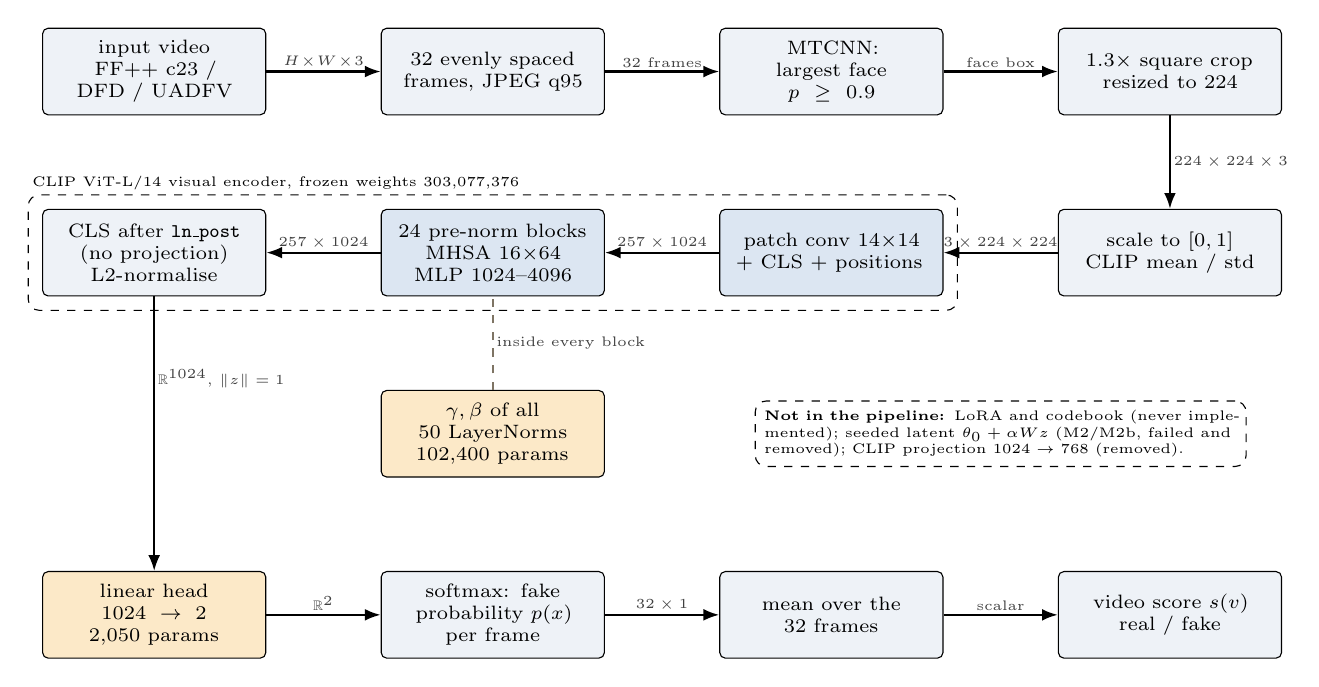
\begin{tikzpicture}[
  x=43mm,y=-23mm,
  blk/.style={draw,rounded corners=2pt,fill=box,align=center,font=\scriptsize,minimum height=11mm,text width=26mm},
  frz/.style={blk,fill=frz},
  trn/.style={blk,fill=trn},
  lab/.style={font=\tiny,text=black!75,inner sep=1pt},
  ar/.style={-{Latex[length=2mm]},thick}]
% row 1: left to right
\node[blk] (vid) at (0,0) {input video\\FF++ c23 / DFD / UADFV};
\node[blk] (frm) at (1,0) {32 evenly spaced\\frames, JPEG q95};
\node[blk] (det) at (2,0) {MTCNN: largest face\\\(p\ge0.9\)};
\node[blk] (crp) at (3,0) {1.3\(\times\) square crop\\resized to 224};
% row 2: right to left
\node[blk] (pre) at (3,1) {scale to \([0,1]\)\\CLIP mean / std};
\node[frz] (pe)  at (2,1) {patch conv 14\(\times\)14\\+ CLS + positions};
\node[frz] (tr)  at (1,1) {24 pre-norm blocks\\MHSA 16\(\times\)64\\MLP 1024--4096};
\node[blk] (cls) at (0,1) {CLS after \texttt{ln\_post}\\(no projection)\\L2-normalise};
% row 3
\node[trn] (ln)  at (1,2) {\(\gamma,\beta\) of all\\50 LayerNorms\\102,400 params};
\node[draw,dashed,rounded corners,font=\tiny,align=left,text width=60mm] at (2.5,2)
 {\textbf{Not in the pipeline:} LoRA and codebook (never implemented); seeded latent \(\theta_0+\alpha Wz\) (M2/M2b, failed and removed); CLIP projection \(1024\to768\) (removed).};
% row 4: left to right
\node[trn] (head) at (0,3) {linear head\\\(1024\to2\)\\2,050 params};
\node[blk] (sm)   at (1,3) {softmax: fake\\probability \(p(x)\)\\per frame};
\node[blk] (agg)  at (2,3) {mean over the\\32 frames};
\node[blk] (out)  at (3,3) {video score \(s(v)\)\\real / fake};
% arrows and shapes
\draw[ar] (vid)--node[lab,above]{\(H\!\times\!W\!\times\!3\)}(frm);
\draw[ar] (frm)--node[lab,above]{\(32\) frames}(det);
\draw[ar] (det)--node[lab,above]{face box}(crp);
\draw[ar] (crp)--node[lab,right]{\(224\times224\times3\)}(pre);
\draw[ar] (pre)--node[lab,above]{\(3\times224\times224\)}(pe);
\draw[ar] (pe)--node[lab,above]{\(257\times1024\)}(tr);
\draw[ar] (tr)--node[lab,above]{\(257\times1024\)}(cls);
\draw[ar] (cls)--node[lab,right,pos=0.3]{\(\mathbb{R}^{1024}\), \(\|z\|=1\)}(head);
\draw[ar] (head)--node[lab,above]{\(\mathbb{R}^{2}\)}(sm);
\draw[ar] (sm)--node[lab,above]{\(32\times1\)}(agg);
\draw[ar] (agg)--node[lab,above]{scalar}(out);
\draw[thick,dashed,trn!50!black] (ln)--node[lab,right]{inside every block}(tr);
\begin{scope}[on background layer]
\node[draw,dashed,rounded corners,fit=(pe)(tr)(cls),inner sep=5pt] (bb) {};
\end{scope}
\node[font=\tiny,anchor=south west,inner sep=1.5pt] at (bb.north west) {CLIP ViT-L/14 visual encoder, frozen weights 303,077,376};
\end{tikzpicture}
\caption{Implemented inference pipeline with tensor shapes. Orange: the only trained parameters, 50 LayerNorms + head = 104,450 numbers (the deployed \(\theta_s\)); blue: frozen. During training, augmentation is applied between cropping and normalisation.}\label{fig:pipeline}
\end{figure}

\begin{figure}[H]\centering
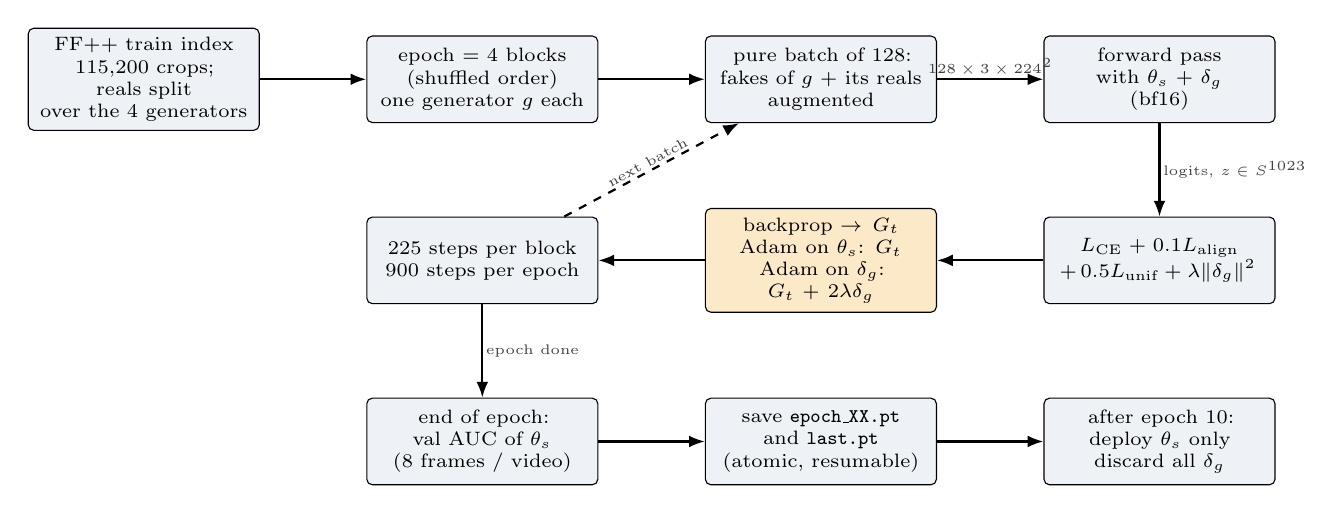
\begin{tikzpicture}[
  x=43mm,y=-23mm,
  blk/.style={draw,rounded corners=2pt,fill=box,align=center,font=\scriptsize,minimum height=11mm,text width=27mm},
  trn/.style={blk,fill=trn},
  lab/.style={font=\tiny,text=black!75,inner sep=1pt},
  ar/.style={-{Latex[length=2mm]},thick}]
\node[blk] (ds)   at (0,0) {FF++ train index\\115,200 crops; reals split\\over the 4 generators};
\node[blk] (blk)  at (1,0) {epoch = 4 blocks\\(shuffled order)\\one generator \(g\) each};
\node[blk] (bat)  at (2,0) {pure batch of 128:\\fakes of \(g\) + its reals\\augmented};
\node[blk] (fw)   at (3,0) {forward pass\\with \(\theta_s+\delta_g\)\\(bf16)};
\node[blk] (loss) at (3,1) {\(L_\text{CE}+0.1L_\text{align}\)\\\(+\,0.5L_\text{unif}+\lambda\|\delta_g\|^2\)};
\node[trn] (bp)   at (2,1) {backprop \(\to G_t\)\\Adam on \(\theta_s\): \(G_t\)\\Adam on \(\delta_g\): \(G_t+2\lambda\delta_g\)};
\node[blk] (nxt)  at (1,1) {225 steps per block\\900 steps per epoch};
\node[blk] (val)  at (1,2) {end of epoch:\\val AUC of \(\theta_s\)\\(8 frames / video)};
\node[blk] (ck)   at (2,2) {save \texttt{epoch\_XX.pt}\\and \texttt{last.pt}\\(atomic, resumable)};
\node[blk] (fin)  at (3,2) {after epoch 10:\\deploy \(\theta_s\) only\\discard all \(\delta_g\)};
\draw[ar] (ds)--(blk); \draw[ar] (blk)--(bat);
\draw[ar] (bat)--node[lab,above]{\(128\times3\times224^2\)}(fw);
\draw[ar] (fw)--node[lab,right]{logits, \(z\in S^{1023}\)}(loss);
\draw[ar] (loss)--(bp); \draw[ar] (bp)--(nxt);
\draw[ar,dashed] (nxt)--node[lab,above,sloped]{next batch}(bat);
\draw[ar] (nxt)--node[lab,right]{epoch done}(val);
\draw[ar] (val)--(ck); \draw[ar] (ck)--(fin);
\end{tikzpicture}
\caption{GBLA training workflow (M4 onward). With \(\lambda=\infty\) the offsets stay zero, which is pooled training with pure-generator batches; M1 used mixed batches and no offsets. No checkpoint is selected by validation or test performance.}\label{fig:training}
\end{figure}

% =====================================================================
\section{Research Contributions}\label{sec:contrib}
% =====================================================================
\subsection{Implemented and verified}
\begin{itemize}
\item A resume-safe, leakage-controlled FF++ c23 pipeline with shared real/fake crop boxes and
official splits (192,000 crops), and matching DFD and UADFV pipelines.
\item A faithful LNCLIP-DF reproduction (within 0.8 AUC points of the paper on six test sets) with
exact parameter accounting (104,450 trainable of 303,181,826).
\item A measurement of generator dominance in pooled LN tuning: Face2Face carries weight 0.58,
NeuralTextures \(\approx0\), \(G_\text{eff}/G=0.57\); NT is under-weighted in all 14 subsets that contain it.
\item GBLA: shared-plus-private optimisation with pure-generator batching, deploying the same 104,450
parameters. Under a fixed 10-epoch budget it improves FaceShifter (92.91 vs 90.53 same-batching
pooled vs 88.19 M1), LOGO mean (+0.55) and DFD (+0.82 over M1, interval excluding 0).
\end{itemize}
\subsection{Preliminary findings (need seeds and more data)}
\begin{itemize}
\item The \(\lambda\) ordering on FF++ FaceShifter carries over to DFD; it does not on UADFV (ceiling).
\item GBLA beats a post-hoc Fisher merge of specialists by 2.70 points on LOGO mean, suggesting that
joint training with offsets does something a merge does not.
\item Pure-generator batching alone changes the generalisation profile (+2.3 FSh, \(-6.0\) NT vs M1).
\end{itemize}
\subsection{Exploratory or theoretical only}
\begin{itemize}
\item Curvature/random-effects interpretation of \(\lambda\) (failed checks).
\item Compact seeded latent (failed), Mapping-Network-style generation, LoRA vs LN comparison,
real-only training, codebook/manifold methods: not implemented or abandoned.
\end{itemize}
\subsection{Unresolved questions}
\begin{itemize}
\item Is the GBLA gain larger than seed variance? (single seed everywhere)
\item Why does GBLA hurt held-out NeuralTextures, the hardest generator?
\item Does the gain persist on harder benchmarks (Celeb-DF v2, DFDC, FFIW, DeepSpeak)?
\item How much of the gain comes from batching vs offsets on other datasets?
\end{itemize}
\textbf{Independent assessment.} \emph{Parameter efficiency}: demonstrated in the sense of
trainable/stored parameters (0.0345\%), inherited from LN tuning; GBLA adds none at deployment but
5\(\times\) at training time; inference cost unchanged. \emph{Detection performance}: in-domain
FF++ AUC is near saturation for all methods and does not discriminate. \emph{Generalisation}: measured
only by unseen-generator and cross-dataset AUC, never by validation accuracy; gains are modest
(0.5--2.4 points) and single-seed.

% =====================================================================
\section{Limitations}\label{sec:limits}
% =====================================================================
\begin{itemize}
\item One seed per configuration; no variance estimate over training randomness (bootstrap intervals
cover only test sampling).
\item MTCNN without landmark alignment at 224 px instead of the paper's RetinaFace alignment at 256 px.
\item FF++ validation saturates; no informative validation set is used for model selection (final
epoch used everywhere).
\item \(\lambda\) was chosen on FaceShifter test AUC in M4 (the only knob tuned this way) and then
fixed for M5--M9b; strictly, FaceShifter is not an untouched test set for the choice of \(\lambda\).
\item Only two cross-dataset benchmarks, one of them at ceiling.
\item Frame-level model; temporal information and patch tokens are discarded.
\item The frozen 303 M backbone dominates inference cost; no compute or latency was measured.
\end{itemize}

% =====================================================================
\section{Motivation for Architectural Redesign}\label{sec:redesign}
% =====================================================================
\textbf{Worth retaining.} The data pipeline and its integrity checks; the frozen-backbone, small-trainable-set
paradigm with full parameter accounting; the evaluation protocol (LOGO, cross-dataset, cluster bootstrap,
paired differences, load checks).

\textbf{Needs modification.} Batching and balancing across generators (the strongest single lever found,
with a cost on NT); validation and model selection (FF++ val is uninformative); number of seeds.

\textbf{To reconsider.} Whether a CLS-only, frame-level representation can carry manipulation evidence
for local edits such as NeuralTextures; whether LayerNorm tuning is the right adaptation structure (the
LN-vs-LoRA question was never tested).

\textbf{Missing evaluations.} Celeb-DF v2 and other harder datasets; robustness (compression, resizing);
compute/latency; multiple seeds; ablation separating batching from offsets on cross-dataset data.

\textbf{Possible overfitting sources.} 1:4 real:fake imbalance; FF++-specific compression (JPEG q95
frames); identity overlap between real and fake in FF++ (controlled by pairing, but identities repeat
across frames); selection of \(\lambda\) on FaceShifter.

\textbf{Questions the redesign must answer.} (1) How to improve held-out NT-like local manipulations
without losing the FaceShifter gain. (2) How to select hyper-parameters without an unseen test set.
(3) Whether gains survive multiple seeds and harder datasets at the same trainable budget.
This report does not propose the new architecture.

% =====================================================================
\section{Future Research Roadmap}\label{sec:roadmap}
% =====================================================================
All items are future work.
\begin{enumerate}
\item Architecture redesign (scope to be agreed with the supervisor).
\item Statistical validation: 3--5 seeds for M1, \(\lambda=\infty\) and \(\lambda=0.01\).
\item Cross-dataset testing on Celeb-DF v2 (download notebook prepared outside the repository), DFDC,
FFIW, DeepSpeak.
\item Ablations: batching vs offsets; \(\lambda\) chosen without FaceShifter; adapter structure (LN vs
LoRA at matched parameter count).
\item Parameter-efficiency comparison including inference compute and memory.
\item Additional manipulation types (DF40-style face swaps, diffusion-based).
\item Robustness evaluation (JPEG, resizing, blur).
\item Reproducibility package: scripts extracted from notebooks, fixed environment file.
\end{enumerate}

% =====================================================================
\begin{thebibliography}{99}\small
\bibitem{tian2023unsupervised} M.~Tian, M.~Khayatkhoei, J.~Mathai, W.~AbdAlmageed. Unsupervised Multimodal Deepfake Detection Using Intra- and Cross-Modal Inconsistencies. arXiv:2311.17088, 2023. Later version: BMVC 2025. \url{https://arxiv.org/abs/2311.17088}
\bibitem{sen2026mapping} L.~Sen, S.~Mukherjee. Mapping Networks. CVPR 2026 (paper PDF in the thesis folder).
\bibitem{wang2026breaking} C.~Wang, J.~Wang, K.-Y.~Zhang, T.~Yao, S.~Ding, R.~Yi, L.~Ma. Breaking Manifold Continuity: Vector Quantized Modeling for Real-Centric Deepfake Detection. Proc.\ 43rd ICML, PMLR, 2026.
\bibitem{zhao2026casoadd} Y.~Zhao, K.~Zhang, Z.~Hua, Y.~Zhang, Q.~Liao, W.~Jiang. Learning Tight Rejection Boundaries without Negatives for Strict One-Class Audio Deepfake Detection. Proc.\ 43rd ICML, PMLR, 2026.
\bibitem{yermakov2025lnclip} A.~Yermakov, J.~Cech, J.~Matas, M.~Fritz. Deepfake Detection that Generalizes Across Benchmarks. arXiv:2508.06248, 2025 (recorded in M1 as WACV 2026). Code: \url{https://github.com/yermandy/GenD}
\bibitem{yermakov2025unlocking} A.~Yermakov, J.~Cech, J.~Matas. Unlocking the Hidden Potential of CLIP in Generalizable Deepfake Detection. arXiv:2503.19683, 2025.
\bibitem{radford2021clip} A.~Radford et al. Learning Transferable Visual Models From Natural Language Supervision. ICML 2021.
\bibitem{rossler2019ffpp} A.~R\"ossler et al. FaceForensics++: Learning to Detect Manipulated Facial Images. ICCV 2019.
\bibitem{li2020faceshifter} L.~Li et al. FaceShifter: Towards High Fidelity and Occlusion Aware Face Swapping. arXiv:1912.13457, 2020.
\bibitem{yang2019uadfv} X.~Yang, Y.~Li, S.~Lyu. Exposing Deep Fakes Using Inconsistent Head Poses. ICASSP 2019 (UADFV).
\bibitem{zhang2016mtcnn} K.~Zhang, Z.~Zhang, Z.~Li, Y.~Qiao. Joint Face Detection and Alignment Using Multitask Cascaded Convolutional Networks. IEEE Signal Processing Letters, 2016.
\bibitem{wang2020alignment} T.~Wang, P.~Isola. Understanding Contrastive Representation Learning through Alignment and Uniformity on the Hypersphere. ICML 2020.
\bibitem{hu2022lora} E.~J.~Hu et al. LoRA: Low-Rank Adaptation of Large Language Models. ICLR 2022.
\bibitem{li2018intrinsic} C.~Li, H.~Farkhoor, R.~Liu, J.~Yosinski. Measuring the Intrinsic Dimension of Objective Landscapes. ICLR 2018.
\bibitem{aghajanyan2021intrinsic} A.~Aghajanyan, S.~Gupta, L.~Zettlemoyer. Intrinsic Dimensionality Explains the Effectiveness of Language Model Fine-Tuning. ACL 2021.
\bibitem{nooralinejad2023pranc} P.~Nooralinejad et al. PRANC: Pseudo RAndom Networks for Compacting Deep Models. ICCV 2023.
\bibitem{koohpayegani2024nola} S.~A.~Koohpayegani et al. NOLA: Compressing LoRA using Linear Combination of Random Basis. ICLR 2024.
\bibitem{khosla2012undoing} A.~Khosla, T.~Zhou, T.~Malisiewicz, A.~A.~Efros, A.~Torralba. Undoing the Damage of Dataset Bias. ECCV 2012.
\bibitem{evgeniou2004multitask} T.~Evgeniou, M.~Pontil. Regularized Multi-Task Learning. KDD 2004.
\bibitem{piratla2020csd} V.~Piratla, P.~Netrapalli, S.~Sarawagi. Efficient Domain Generalization via Common-Specific Low-Rank Decomposition. ICML 2020. arXiv:2003.12815.
\bibitem{matena2022fisher} M.~Matena, C.~Raffel. Merging Models with Fisher-Weighted Averaging. NeurIPS 2022. arXiv:2111.09832.
\bibitem{kish1965} L.~Kish. Survey Sampling. Wiley, 1965.
\bibitem{dersimonian1986meta} R.~DerSimonian, N.~Laird. Meta-Analysis in Clinical Trials. Controlled Clinical Trials, 1986.
\bibitem{gulrajani2021domainbed} I.~Gulrajani, D.~Lopez-Paz. In Search of Lost Domain Generalization. ICLR 2021.
\end{thebibliography}
\textit{Note.} Entries for papers 4--8 were checked against the PDFs in the thesis folder; Tian et al.\
against arXiv. Standard references (CLIP, FF++, LoRA, etc.) are cited as recorded in the project and
should be checked for page numbers before external submission.

% =====================================================================
\appendix
\section{Notation}
\begin{table}[H]\centering\small
\caption{Symbols.}
\begin{tabularx}{\linewidth}{@{}lY@{}}
\toprule
Symbol & Meaning\\
\midrule
\(x, y, g\) & face crop; label (1 = fake); generator\\
\(\mathcal{G}, G\) & training generators; their number (4 in the standard protocol)\\
\(P\) & adapted parameters: 102,400 LayerNorm + 2,050 head = 104,450\\
\(\theta_0,\theta_s,\delta_g\) & initial values; shared parameters (deployed); private offset of \(g\) (training only)\\
\(\lambda\) & strength of the offset penalty\\
\(v_g\) & solution of LN tuning on generator \(g\) alone (M3, M6)\\
\(w_g, G_\text{eff}\) & geometric weight of \(g\) in the pooled solution; Kish effective number\\
\(z(x)\) & L2-normalised CLS feature, \(\mathbb{R}^{1024}\)\\
\(W, z, \alpha, d\) & (M2/M2b only) seeded random matrix, latent, scale, latent size\\
\bottomrule
\end{tabularx}
\end{table}

\section{Full M7 subset table}
\begin{table}[H]\centering\scriptsize
\caption{M7: geometric \(G_\text{eff}\), share of the pooled direction explained by the single-generator directions, seen AUC and mean OOD AUC for all 25 subsets.}
\begin{tabular}{@{}lrrrrr|lrrrrr@{}}
\toprule
Subset & \(|S|\) & \(G_\text{eff}/|S|\) & Expl. & Seen & OOD & Subset & \(|S|\) & \(G_\text{eff}/|S|\) & Expl. & Seen & OOD\\
\midrule
DF+F2F+FS+NT & 4 & 0.659 & 0.660 & 96.41 & 90.53 & F2F+FS+FSh & 3 & 0.985 & 0.726 & 99.25 & 80.20\\
DF+F2F+FS+FSh & 4 & 0.979 & 0.705 & 99.15 & 64.40 & F2F+NT+FSh & 3 & 0.531 & 0.724 & 95.55 & 98.37\\
DF+F2F+NT+FSh & 4 & 0.628 & 0.702 & 95.01 & 97.90 & FS+NT+FSh & 3 & 0.689 & 0.736 & 90.91 & 92.29\\
DF+FS+NT+FSh & 4 & 0.715 & 0.713 & 91.94 & 85.40 & DF+F2F & 2 & 0.983 & 0.736 & 99.37 & 86.47\\
F2F+FS+NT+FSh & 4 & 0.604 & 0.697 & 94.42 & 99.21 & DF+FS & 2 & 0.963 & 0.796 & 99.86 & 78.48\\
DF+F2F+FS & 3 & 0.981 & 0.739 & 99.46 & 80.44 & DF+NT & 2 & 0.854 & 0.680 & 96.63 & 92.18\\
DF+F2F+NT & 3 & 0.607 & 0.709 & 96.84 & 92.43 & DF+FSh & 2 & 0.975 & 0.776 & 99.79 & 77.29\\
DF+F2F+FSh & 3 & 0.998 & 0.723 & 99.01 & 83.02 & F2F+FS & 2 & 1.000 & 0.742 & 99.35 & 83.11\\
DF+FS+NT & 3 & 0.871 & 0.745 & 94.04 & 92.95 & F2F+NT & 2 & 0.635 & 0.725 & 96.06 & 91.67\\
DF+FS+FSh & 3 & 0.996 & 0.770 & 99.60 & 68.89 & F2F+FSh & 2 & 1.000 & 0.734 & 99.12 & 87.27\\
DF+NT+FSh & 3 & 0.727 & 0.686 & 92.13 & 90.48 & FS+NT & 2 & 0.807 & 0.706 & 95.63 & 94.24\\
F2F+FS+NT & 3 & 0.601 & 0.737 & 95.36 & 93.44 & FS+FSh & 2 & 0.999 & 0.765 & 99.67 & 78.30\\
 & & & & & & NT+FSh & 2 & 0.812 & 0.720 & 94.03 & 90.20\\
\bottomrule
\end{tabular}
\end{table}

\section{DFD per-scene and sensitivity results}
\begin{table}[H]\centering\small
\caption{DFD sensitivity (video AUC \%).}
\begin{tabularx}{\linewidth}{@{}lRRR@{}}
\toprule
Model & All videos & Without two-person scenes (3,114 videos) & Single-face frames (80.1\% of crops)\\
\midrule
LNCLIP-DF reproduction (M1) & 95.88 & 97.49 & 96.44\\
Pooled, \(\lambda=\infty\) & 96.05 & 97.65 & 96.43\\
GBLA \(\lambda=1\) & 96.40 & 98.08 & 96.85\\
GBLA \(\lambda=0.1\) & 96.70 & 98.39 & 97.07\\
GBLA \(\lambda=0.01\) & 96.71 & 98.35 & 97.07\\
GBLA \(\lambda=0.001\) & 95.33 & 96.41 & 95.74\\
GBLA \(\lambda=0\) & 94.43 & 95.45 & 94.74\\
Uniform merge & 92.68 & 93.87 & 92.84\\
Fisher merge & 94.95 & 96.36 & 95.19\\
\bottomrule
\end{tabularx}
\end{table}
The two-person scenes are the hardest for every model (e.g.\ \texttt{meeting\_serious}: M1 60.85,
pooled 61.79, GBLA \(\lambda=0.01\) 72.17).

\section{Parameter arithmetic}
\begin{itemize}
\item Patch embedding \(1024\cdot3\cdot14\cdot14=602{,}112\); class + positional \(1024+257\cdot1024=264{,}192\).
\item Attention per block \(3072\cdot1024+3072+1024^2+1024=4{,}198{,}400\); \(\times24=100{,}761{,}600\).
\item MLP per block \(4096\cdot1024+4096+1024\cdot4096+1024=8{,}393{,}728\); \(\times24=201{,}449{,}472\).
\item LayerNorms \(50\times2\times1024=102{,}400\); head \(2\cdot1024+2=2{,}050\).
\item Detector total \(201{,}449{,}472+100{,}761{,}600+602{,}112+264{,}192+102{,}400+2{,}050=303{,}181{,}826\).
\item Tower without head and projection \(303{,}179{,}776\); with projection \(1024\times768=786{,}432\): \(303{,}966{,}208\).
\item GBLA training store \(5\times104{,}450=522{,}250\).
\end{itemize}

\section{Git history}
\begin{table}[H]\centering\scriptsize
\caption{Repository commits (oldest first).}
\begin{tabularx}{\linewidth}{@{}lL{1.6cm}Y@{}}
\toprule
Commit & Date & Message (abridged)\\
\midrule
2572354 & 2026-10-05 & Initial code added\\
83cd5dc & 2026-10-08 & M0 data pre processing pipeline done\\
3e62dfe & 2026-10-13 & reproduce LNCLIP-DF on FF++ c23 (frozen CLIP ViT-L/14, train only \dots)\\
dfc41db & 2026-10-14 & generate the LayerNorm + head parameters as theta = theta0 + alpha*W*z \dots\ sweep latent size d (16--4096)\\
6549a0e & 2026-10-15 & Revised m2 plans in m2b\\
9f1d12d & 2026-10-17 & E1 go/no-go on pooled-training generator dominance\\
0ef0d1f & 2026-10-18 & GBLA shared LayerNorm+head parameters with private offsets\\
0731e63 & 2026-10-19 & leave-one-generator-out for GBLA at lambda 0.01\\
04aa840 & 2026-10-19 & Fisher merging baseline for LOGO comparison\\
5ef28c8 & 2026-10-20 & G\_eff law over 25 generator subsets\\
7a6758d & 2026-10-20 & m7 output analysis\\
439e77a & 2026-11-04 & Cross Dataset Testing 1 on DFD dataset (M8a preprocessing)\\
6661977 & 2026-11-04 & Cross Dataset Testing 1 on DFD dataset\\
f8f6bb7 & 2026-11-05 & Cross Dataset Testing 2 Preprocessing of UADFV dataset\\
06aedba & 2026-11-05 & Cross Dataset Testing 2 on UADFV dataset done\\
\bottomrule
\end{tabularx}
\end{table}

\section{Additional figures}
\begin{figure}[H]\centering
\includegraphics[width=0.62\linewidth]{\figdir/M8b_c24_1.png}
\caption{M8b: video-level ROC curves on DFD.}
\end{figure}

\end{document}
